% CVPR 2024 Paper Template; see https://github.com/cvpr-org/author-kit

\documentclass[10pt,twocolumn,letterpaper]{article}

%%%%%%%%% PAPER TYPE  - PLEASE UPDATE FOR FINAL VERSION
\usepackage{cvpr}              % To produce the CAMERA-READY version
% \usepackage[review]{cvpr}      % To produce the REVIEW version 
% \usepackage[pagenumbers]{cvpr} % To force page numbers, e.g. for an arXiv version
\usepackage[accsupp]{axessibility}

% Import additional packages in the preamble file, before hyperref
%
% --- inline annotations
%
\newcommand{\red}[1]{{\color{red}#1}}
\newcommand{\todo}[1]{{\color{red}#1}}
\newcommand{\TODO}[1]{\textbf{\color{red}[TODO: #1]}}
% --- disable by uncommenting  
% \renewcommand{\TODO}[1]{}
% \renewcommand{\todo}[1]{#1}




\definecolor{cvprblue}{rgb}{0.21,0.49,0.74}
\usepackage[pagebackref,breaklinks,color links,citecolor=cvprblue]{hyperref}
\usepackage{makecell}
\usepackage{multirow, multicol}
\usepackage{adjustbox}
\usepackage{boldline}
% \usepackage{amssymb}%
% \usepackage{amsmath}
% \usepackage{multirow}%multiraw
\usepackage{pifont}%xmark
\newcommand{\xmark}{\ding{55}}
\newcommand{\cmark}{\ding{51}}
\usepackage{array}
\usepackage{multirow}
\usepackage{makecell}
\usepackage{tabularray}
\usepackage{algorithmic}
\usepackage[accsupp]{axessibility}
\usepackage{algorithm}
\usepackage{colortbl}  % 表格颜色
\usepackage{xcolor}  % 颜色宏包
\usepackage{amsthm}

% \usepackage{hyperref}
\linespread{1.0}
% \newcommand{\jw}[1]{{\color[rgb]{1.0,0.0,0.0}{[JW:#1]}}}
%%%%%%%%% PAPER ID  - PLEASE UPDATE
\def\paperID{1021} % *** Enter the Paper ID here
\def\confName{CVPR}
\def\confYear{2025}
% \newcommand{\dong}[1]{\textcolor{red}{#1}}
\newcommand{\pb}[1]{{\color[rgb]{1.0,0.0,0.0}{[PB:#1]}}}

% \title{Universe Learning for Test-time Domain Generalization: A Multi-Matching Approach to Medical Image Segmentation}

\title{Test-Time Domain Generalization via Universe Learning: A Multi-Graph Matching Approach for Medical Image Segmentation}
% \title{From Multi-Matching to Test-Time Domain Generalization: An Universe Representation for Medical Image Segmentation}

%%%%%%%%% AUTHORS - PLEASE UPDATE

\author{Xingguo Lv\textsuperscript{1,2}~ Xingbo Dong\textsuperscript{1}\footnotemark[2] ~ Liwen Wang\textsuperscript{1} ~ Jiewen Yang\textsuperscript{3} ~ Lei Zhao\textsuperscript{2}\\  Bin Pu\textsuperscript{3}\footnotemark[2] ~ Zhe Jin\textsuperscript{1} ~ Xuejun Li\textsuperscript{1}\\
\textsuperscript{1} Anhui Provincial International Joint Research Center for Advanced Technology in Medical Imaging,\\ Anhui University.
\textsuperscript{2} Hunan University.
\textsuperscript{3} The Hong Kong University of Science and Technology.\\
{\tt\small lvxg@stu.ahu.edu.cn, xingbo.dong@ahu.edu.cn, eebinpu@ust.hk}
}

\begin{document}
\maketitle
\begin{abstract}
Fine-tuning provides an effective means to specialize pre-trained models for various downstream tasks. However, fine-tuning often incurs high memory overhead, especially for large transformer-based models, such as LLMs. While existing methods may reduce certain parts of the memory required for fine-tuning, they still require caching all intermediate activations computed in the forward pass to update weights during the backward pass. In~this work, we develop \method, a method to reduce memory usage,  specifically the memory to store intermediate activations, in the fine-tuning of transformer-based models. During the backward pass, \method approximates the gradient computation by backpropagating through just a subset of input tokens. Thus, with \method, only a subset of intermediate activations are cached during the forward pass. Also, \method can be easily combined with existing methods like LoRA, further reducing the memory cost. We evaluate our approach on pre-trained transformer models with up to billions of parameters, considering the performance on multiple downstream tasks such as text classification and question answering in a few-shot learning setup. Overall, \method achieves performance on par with full fine-tuning or representative memory-efficient fine-tuning methods,  while greatly reducing the memory footprint, especially when combined with other methods with complementary memory reduction mechanisms. We hope that our approach will facilitate the fine-tuning of large transformers,  in specializing them for specific domains or co-training them with other neural components from a larger system. Our code is available at \githubURL.
\blfootnote{\textbf{*} Equal contribution}
\end{abstract}

\section{Introduction}
\label{sec:intro}

\begin{figure*}[t!]
    \centering
    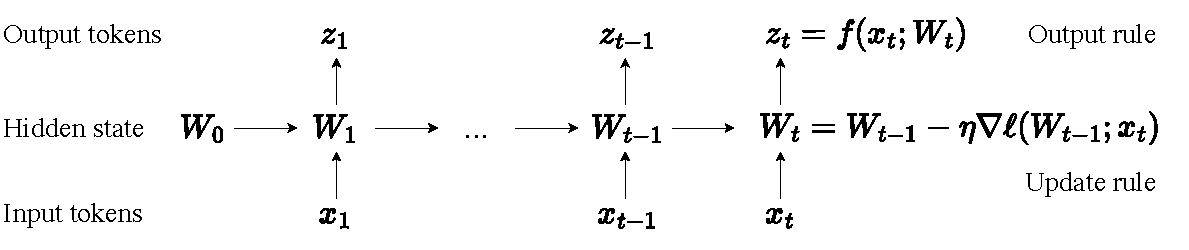
\includegraphics[width=0.8\textwidth]{figs/simple_teaser.pdf}
    \caption{All RNN layers can be expressed as a hidden state that transitions according to an update rule.
    The key idea in \cite{sun2024ttt} is to make the hidden state itself a model $f$ with weights $W$, and the update rule a gradient step on the self-supervised loss $\ell$.
    Therefore, updating the hidden state on a test sequence is equivalent to training the model $f$ at test time. 
    This process, known as Test-Time Training (TTT), is programmed into TTT layers. 
    Figure and caption taken from \cite{sun2024ttt}.
    }
    \label{fig:ttt-layer}
\end{figure*}

Despite the remarkable progress in visual and physical realism, state-of-the-art video Transformers are still generating mostly short clips of single scenes without complex stories.
At the time of writing (March 2025), the maximum length of public APIs for video generation is 20 seconds for Sora (OpenAI), 16 seconds for MovieGen (Meta), 10 for Ray~2 (Luma), and 8 for Veo~2 (Google).
None of these APIs can autonomously generate complex multi-scene stories.

A fundamental challenge behind these technical limitations is long context, because the cost of self-attention layers in Transformers increases quadratically with context length.
This challenge is especially acute for video generation with dynamic motion, whose context cannot be easily compressed by a tokenizer.
Using a standard tokenizer, each of our one-minute videos requires over 300k tokens in context. 
With self-attention, generating a one-minute video would have taken $11\times$ longer than generating 20 videos of 3 seconds each, and training would have taken $12\times$ longer.

To address this challenge, recent work on video generation has investigated RNN layers as an efficient alternative to self-attention, because their cost increases linearly with context length~\cite{wang2024lingenhighresolutionminutelengthtexttovideo}.
Modern RNN layers, especially variants of linear attention~\cite{schmidhuberlinearattn, katharopoulos2020lineartransformers} such as Mamba~\cite{gu2024mamba, dao2024mamba2} and DeltaNet~\cite{schlag2021deltanet, yang2025gateddeltanetworksimproving}, have shown impressive results for natural language tasks.
However, we have yet to see long videos with complex stories or dynamic motion generated by RNNs.
Videos (\href{https://lineargen.github.io/}{link}) in \cite{wang2024lingenhighresolutionminutelengthtexttovideo} are high resolution and one-minute long, but contain only single scenes and slow motion, let alone complex stories.

We believe that these RNN layers generate less complex videos because their hidden states are less expressive.
RNN layers can only store past tokens into a hidden state of fixed size, which is only a matrix for linear attention variants such as Mamba and DeltaNet.
It is inherently challenging to compress hundreds of thousands of vectors into a matrix with only thousands in rank.
As a consequence, these RNN layers struggle to remember the deep relationships between distant tokens.

We experiment with an alternative class of RNN layers whose hidden states themselves can be neural networks. Specifically, we use two-layer MLPs with 2$\times$ more hidden cells and richer nonlinearities than the linear (matrix) hidden states in linear attention variants.
Since the neural network hidden states are updated by training even on test sequences, these new layers are called Test-Time Training (TTT) layers~\cite{sun2024ttt}.

We start from a pre-trained Diffusion Transformer (CogVideo-X 5B \cite{hong2023cogvideo}) that could only generate 3-second short clips at 16 fps (or 6 seconds at 8 fps).
Then, we add TTT layers initialized from scratch and fine-tune this model to generate one-minute videos from text storyboards. 
We limit the self-attention layers to 3-second segments so their cost stays manageable.
With only preliminary systems optimization, our training run takes the equivalent of 50 hours on 256 H100s.

We curate a text-to-video dataset based on $\approx$ 7 hours of \textit{Tom and Jerry} cartoons with human-annotated storyboards.
We intentionally limit our scope to this specific domain for fast research iteration.
As a proof-of-concept, our dataset emphasizes complex, multi-scene, and long-range stories with dynamic motion, where progress is still needed; it has less emphasis on visual and physical realism, where remarkable progress has already been made.
We believe that improvements in long-context capabilities for this specific domain will transfer to general-purpose video generation.

Compared to strong baselines such as Mamba 2~\cite{dao2024mamba2}, Gated DeltaNet~\cite{yang2025gateddeltanetworksimproving}, and sliding-window attention layers, TTT layers generate much more coherent videos that tell complex stories with dynamic motion, leading by 34 Elo points in a human evaluation of 100 videos per method.
For context, GPT-4o scores 29 Elo points over GPT-4 Turbo in LMSys Chatbot Arena~\cite{chiang2024chatbot}.

Sample videos, code and annotations are available at:
\url{https://test-time-training.github.io/video-dit}
\section{Related Works}
\label{sec:related}
\subsection{Encoder-based MLLMs}
The dominant architecture of MLLMs has remained largely unchanged since its inception, comprising three components: a ViT \cite{clip, siglip, aimv2}, an LLM \cite{llama, gpt3, qwen2.5, vicuna}, and a connector to bridge modality gaps. Previous research has focused primarily on connector design, ranging from simple MLP layers \cite{llava, llava1_5, minigpt, minigptv2} to hierarchical feature fusion modules \cite{flamingo, llama3.2} or other complex architectures \cite{elysium, dynamicvlm, internvl, cambrian1}. Despite these innovations, fundamental limitations persist due to their reliance on external vision encoders. First, computational and memory overhead escalates dramatically when applying multiple vision encoders \cite{cambrian1} or scaling to larger ones \cite{cogvlm}. Second, fixed-resolution pre-training of ViTs forces MLLMs to employ workarounds like image tiling \cite{llava1_5, llavaov} or restricted square resolutions \cite{cogvlm, qwen}. Recent attempts \cite{pixtral, qwen2vl, aimv2} to train resolution-agnostic ViTs have remained impractical, in that they adopted massive proprietary data and opaque training procedures. These challenges have spurred interest in encoder-free architectures that could bypass ViTs entirely.
\subsection{Encoder-free MLLMs}
The pioneering work, Fuyu \cite{fuyu}, demonstrated the feasibility of training encoder-free models on interleaved image-text data, though at prohibitive computational costs with limited technical transparency. Subsequent approaches, such as EVE \cite{eve}, reduced the vision encoder parameters to a single Transformer block, aligning its output features with a ViT through distillation while updating all LLM parameters to learn about vision during the main training stage. However, these methods still struggle with conflicts between the LLM’s inherent language abilities and the new modality, i.e., vision. These conflicts arise from the coupled language and vision parameters, which exacerbate unstable training and lead to catastrophic forgetting of the original language abilities.
% Fuyu \cite{fuyu} pioneered such an approach by training on interleaved image-text data. However, this method required substantial computational resources and the detailed technic is unavalable. Subsequent efforts, such as EVE \cite{eve}, explored converting pre-trained LLMs into MLLMs by replacing ViTs with a single transformer block and aligning features via a distillation-like method. This can be understood as reducing the parameters of the vision encoder. During their main stage training, all LLM parameters are updated. Such methods have certain issues, where the modality confliction between a well-pretrained LLM and a new modality that LLM has never seen before remains a severe problem that can easily cause the training unstable, and even we can stablize the training, such method suffer from catastropic forgetting issue.

To overcome these problems, Mono-InternVL \cite{monointernvl} and EVEv2 \cite{evev2} proposed parameter decoupling strategies inspired by the MoE method \cite{moe}, duplicating LLM parameters for vision-specific processing while freezing its original weights. Despite successfully addressing forgetting issues and modality conflicts, these methods suffered from substantial memory overhead by doubling model parameters, compromising architectural simplicity. 
% This tension highlights a critical insight: preserving LLM integrity while integrating vision understanding requires strict parameter decoupling without persistent duplication. 
Our work addresses this by applying LoRA, which encodes vision while maintaining the language abilities of the LLM, and can be merged into the LLM without causing additional memory overhead.
%while maintaining modality alignment.


% \subsection{Encoder-based MLLM}
% The mainstream architecture of MLLMs follows the “Vision-Connector-LLM” framework, consisting of three key components: the vision encoder(s), the connector, and the LLM. Below, we examine these components in detail.
% \\
% \textbf{vision Encoder}
% The vision encoders used in MLLMs are often trained with contrastive learning loss on image-text tasks, such as CLIP. Additionally, there are other vision encoders trained on vision tasks using self-supervised or semi-supervised objectives. These pre-trained vision encoders provide strong prior knowledge in vision, making them widely adopted in MLLMs.
% \\
% \textbf{Connector}
% Due to the misalignment between the semantic spaces of vision encoders and LLMs, a connector is typically required to bridge this gap, which is one of the most distinctive functions of the connector. Its architecture can vary based on its additional functions, such as re-sampling to reduce the number of visual tokens.
% \\
% \textbf{LLM}
% The LLM often serves as the core component of the architecture, consuming the majority of computations and parameters. These models are typically developed by large companies or organizations due to the substantial amounts of data and training costs involved. The open community usually focuses on post-training enhancements or develops MLLMs based on existing LLMs.
% \subsection{\mono}
% We define \mono as utilizing a single Transformer, specifically an LLM, to perform multimodal tasks. This architecture requires only a few parameters to convert the dimensionality of data from other modalities, such as using a patchifier for vision, without the need for additional pre-trained models. The explorations of this kind of architecture emerges quite early, but soon struggles in several problems caused by the big gap between 
\section{Method}
\label{sec:method}
Our approach, in line with previous methods, builds upon a pre-trained VLM, CLIP \cite{clip}. In this section, we detail the construction of our MMRL framework and the implementation specifics.

\subsection{Preliminary}
We begin by defining the notations used in our approach. CLIP comprises two encoders: an image encoder $\mathcal{V}$ and a text encoder $\mathcal{W}$.

\noindent \textbf{Image Encoding:} The image encoder $\mathcal{V}$ consists of $L$ transformer \cite{transformer} layers, denoted $\{\mathcal{V}_i\}_{i=1}^{L}$. Given an input image \( x \in \mathbb{R}^{H \times W \times 3} \), it is divided into \( M \) fixed-size patches, each projected into a patch embedding, resulting in \( E_0 \in \mathbb{R}^{M \times d_v} \), where $M$ represents the number of patches and $d_v$ the embedding dimension. The initial patch embeddings $E_0$ are combined with a learnable class token $c_0$ and positional encodings, forming the input sequence for the transformer layers. Each layer processes this sequence as
\begin{equation}
    [c_i, E_i] = \mathcal{V}_i([c_{i-1}, E_{i-1}]) \quad
    i = 1, 2, \ldots, L
    \nonumber
\end{equation}
After passing through all transformer layers, a patch projection layer, $P_v^c$, projects the output of the class token, $c_L$, into a shared V-L latent space,
\begin{equation}
    f = P_v^c(c_L)
    \nonumber
\end{equation}
where $f \in \mathbb{R}^{d}$.

\noindent \textbf{Text Encoding:} For an input text, \eg, ``A photo of a [CLASS].", it is tokenized and converted into embeddings $T_0 \in \mathbb{R}^{N \times d_t}$, where $N$ is the token length and $d_t$ the embedding dimension. Beginning-of-text (BOT) and end-of-text (EOT) tokens, denoted $b_0$ and $e_0$, mark the sequence boundaries. These token embeddings, with positional encodings, are passed through the text encoder's $L$ transformer layers, $\{\mathcal{W}_i\}_{i=1}^{L}$, as follows,
\begin{equation} 
    [b_i, T_i, e_i] = \mathcal{W}_i([b_{i-1}, T_{i-1}, e_{i-1}]) \quad i = 1, \ldots, L 
    \nonumber
\end{equation} 
After the final layer, the output of the EOT token, $e_L$, is projected into the shared V-L space using $P_t$,
\begin{equation} 
    w = P_{t}(e_{L}) \nonumber
\end{equation} 
where $w \in \mathbb{R}^{d}$.

\noindent \textbf{Classification with CLIP:} With the image feature $f$ and text features $\{w_c\}_{c=1}^C$ for $C$ classes, CLIP calculates the cosine similarity between $f$ and each $w_c$,
\begin{equation} 
    \text{sim}(f, w_c) = \frac{f \cdot w_c}{|f| |w_c|}, \nonumber 
\end{equation} 
where $|\cdot|$ represents the $L_2$ norm. Class probabilities are then computed using the softmax function,
\begin{equation} 
    p(y = c \mid f) = \frac{\exp(\text{sim}(f, w_c) / \tau)}{\sum_{i=1}^{C} \exp(\text{sim}(f, w_i) / \tau)} \nonumber 
\end{equation} 
where $\tau$ is a temperature parameter. The final predicted class is selected as the one with the highest probability score.

% The predicted class $\hat{y}$ is determined by: \begin{equation} 
%     \hat{y} = \arg\max_{c} , p(y = c \mid f). \nonumber
% \end{equation}


%-------------------------------------------------------------------------
\begin{figure*}[tb]
\setlength{\abovecaptionskip}{0.2cm}   %调整图片标题与图距离
\setlength{\belowcaptionskip}{-0.4cm}   %调整图片标题与下文距离
\centering
\setlength{\belowcaptionskip}{-0.39cm}   %调整图片标题与下文距离
  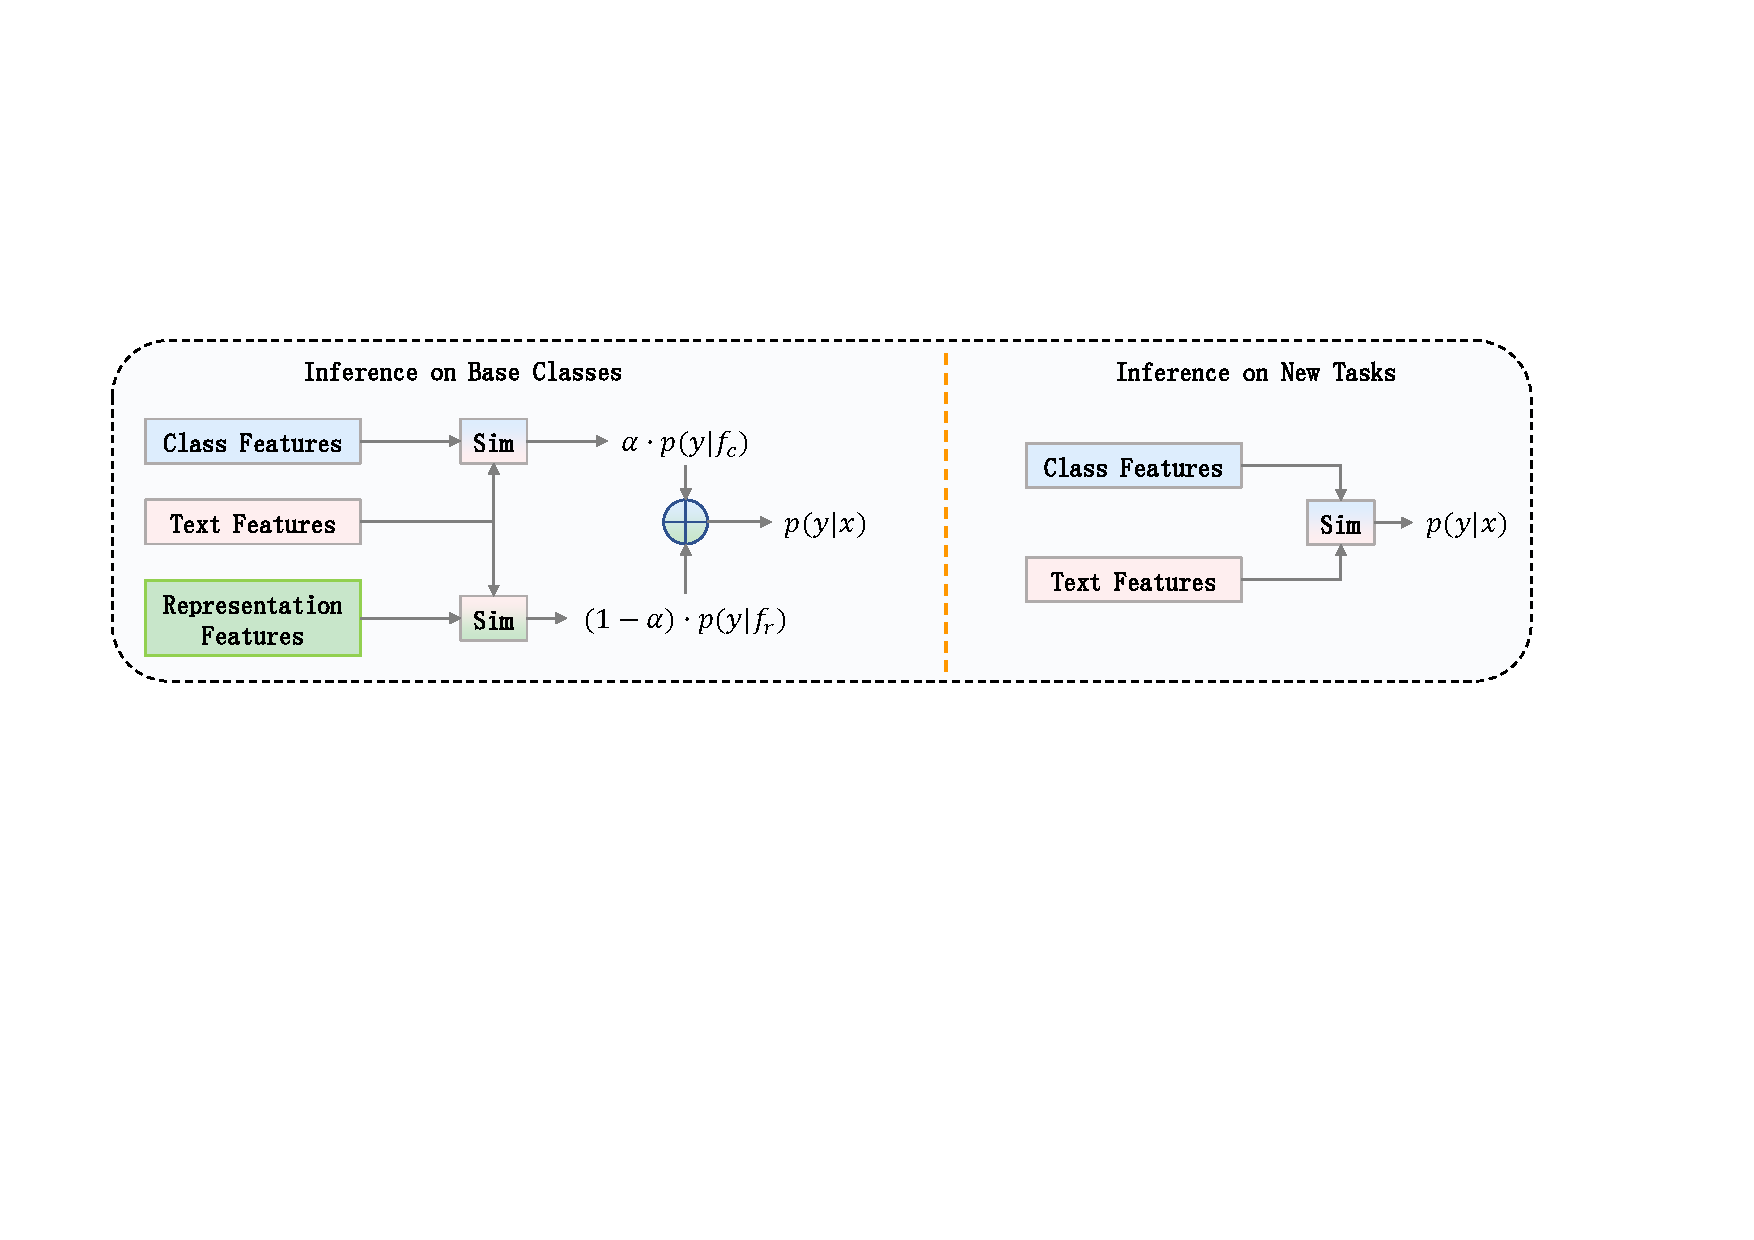
\includegraphics[width=0.7\linewidth]{fig/frame2.pdf}
  \caption{MMRL inference process, where different tasks utilize distinct features.}
  \label{framework2}
\end{figure*}
%-------------------------------------------------------------------------


\subsection{Multi-Modal Representation Learning (MMRL)} Our proposed MMRL aims to address the challenges of adapting pre-trained VLMs using few-shot data while maintaining generalization to new tasks. The training and inference frameworks of MMRL are shown in \cref{framework1} and \cref{framework2}, respectively. In the following, we describe the specifics of the methodology.


\subsubsection{Learnable Representation Space}
MMRL establishes a shared, learnable representation space $\mathcal{R}$ to facilitate multimodal interactions, initialized through sampling from a Gaussian distribution. Using a learnable mapping function $\mathcal{F}(\cdot)$, implemented as a linear layer, we project the tokens $R \in \mathbb{R}^{K \times d_r}$ in this space—where $K$ is the number of tokens and $d_r$ is the dimension of the representation space—into both visual and textual modalities,
\begin{align}
    R^v = \{R_i^v\}_{i=J-1}^{L-1} \quad & R_i^v = \mathcal{F}_i^v(R) \nonumber \\ 
    R^t = \{R_i^t\}_{i=J-1}^{L-1} \quad & R_i^t = \mathcal{F}_i^t(R) \nonumber 
\end{align}
where $R_i^v \in \mathbb{R}^{K \times d_v}$ and $R_i^t \in \mathbb{R}^{K \times d_t}$ represent the representation tokens for visual and textual modalities, respectively, in the $(i+1)$-th transformer layer. The index $J$ indicates the starting layer from which these representation tokens are integrated into the encoders.


\subsubsection{Integration into Higher Encoder Layers}
To preserve the generalized knowledge in the lower layers of the pre-trained CLIP model, the representation tokens $\mathcal{R}^v$ and $\mathcal{R}^t$ are integrated into the higher layers of the image encoder $\mathcal{V}$ and the text encoder $\mathcal{W}$, beginning from the $J$-th layer.


For the image encoder $\mathcal{V}$,
\begin{align}
    [c_i, E_i] &= \mathcal{V}_i([c_{i-1}, E_{i-1}]) \quad i = 1, \ldots, J-1 \nonumber \\  
    [c_i, \_, E_i] &= \mathcal{V}_i([c_{i-1}, R_{i-1}^v, E_{i-1}]) \quad i = J, \ldots, L - 1 \nonumber \\
    [c_i, R_i^v, E_i] &= \mathcal{V}_i([c_{i-1}, R_{i-1}^v, E_{i-1}]) \quad i = L \nonumber
\end{align}

For the text encoder $\mathcal{W}$, while previous prompt learning \cite{maple} involves replacing parts of $T_i$ to incorporate deep prompts, we retain the entire $T_i$ and insert $R_i^t$ before it, aiming to preserve the original textual information,
\begin{align}
    [b_i, T_i, e_i] &= \mathcal{W}_i([b_{i-1}, T_{i-1}, e_{i-1}]) \quad i = 1, \ldots, J-1 \nonumber \\  
    [b_i, \_, T_i, e_i] &= \mathcal{W}_i([b_{i-1}, R_{i-1}^t, T_{i-1}, e_{i-1}]) \nonumber \\
    &\hspace{4cm} i = J, \ldots, L-1 \nonumber \\
    [b_i, R_i^t, T_i, e_i] &= \mathcal{W}_i([b_{i-1}, R_{i-1}^t, T_{i-1}, e_{i-1}]) \quad i = L \nonumber
\end{align}
Note that due to the autoregressive nature of the text encoder, we adjust the attention mask matrix to accommodate the increased embedding length.


\subsubsection{Representation Learning}
Representation learning is designed to leverage representation tokens for dataset-specific adaptation, while the class token preserves the pre-trained knowledge of the original CLIP. Through a set of strategies aimed at retaining generalization during both training and inference, MMRL enables flexible inference for different tasks, as detailed below.


\begin{itemize} 

\item \textbf{Training Phase:} We optimize the features of both the representation tokens and the original class token, with the primary focus on representation features to preserve pre-trained knowledge. Specifically, the projection layer for the representation tokens is trainable, while that for the class token remains fixed. For the image encoder $\mathcal{V}$, after passing through $L$ transformer layers, we obtain the output $c_L \in \mathbb{R}^{d_v}$ for the class token and $R_L^v \in \mathbb{R}^{K \times d_v}$ for the $K$ representation tokens. The final output of the representation tokens, $r_L$, is derived by averaging across the $K$ tokens,
\begin{equation}
    r_L = \text{Mean}(R_L^v) \nonumber
\end{equation}
where $r_L \in \mathbb{R}^{d_v}$. We then apply the patch projection layers to map the outputs of both the class and representation tokens into the common V-L latent space, yielding the class features $f_c$ and representation features $f_r$.
\begin{equation}
    f_c = P_v^c(c_L) \quad f_r = P_v^r(r_L) \nonumber
\end{equation}
Here, $P_v^c$ is the original, frozen patch projection layer of CLIP for class features, while $P_v^r$ for representation features is trainable.

For the text encoder $\mathcal{W}$, following the sequential nature of text, we map the EOT token $e_L$—as in the original CLIP model—after processing through $L$ transformer layers into the common V-L space, yielding the text features.
\begin{equation} 
    w = P_{t}(e_{L}) \nonumber
\end{equation}
With the image features $f_c$, $f_r$, and the text classifiers $\{w_c\}_{c=1}^C$ for $C$ classes, we apply cross-entropy loss to separately optimize the class and representation features,
\begin{align}
\setlength\abovedisplayskip{3pt}
\setlength\belowdisplayskip{3pt}
    \mathcal{L}_{ce}^c &= -\sum_c^C y_c \log p(y = c \mid f_c) \nonumber \\
    \mathcal{L}_{ce}^r &= -\sum_c^C y_c \log p(y = c \mid f_r) \nonumber
\end{align}
where $y_c = 1$ if the image $x$ belongs to class $c$, and $y_c = 0$ otherwise. To further preserve the generalization of class features, we maximize the cosine similarity between $(f_c, w)$ and the frozen CLIP features $(f_0, w_0)$, explicitly guiding the training trajectory,
\begin{equation}
    \mathcal{L}_{cos}^v = 1 - \frac{f_c \cdot f_0}{|f_c| |f_0|} \quad \mathcal{L}_{cos}^t = 1 - \frac{1}{C}\sum_c^C \frac{w^c \cdot w_0^c}{|w^c| |w_0^c|}, \nonumber
\end{equation}
The final MMRL loss function is
\begin{equation}
    \mathcal{L}_{MMRL} = \alpha \mathcal{L}_{ce}^c + (1 - \alpha) \mathcal{L}_{ce}^r + \lambda (\mathcal{L}_{cos}^v + \mathcal{L}_{cos}^t)  \nonumber
\end{equation}
where $\alpha$ controls the balance between the features, and $\lambda$ is the penalty coefficient.

\item \textbf{Testing on Base Classes:} 
For in-distribution classes seen during training, we combine the dataset-specific representation features with the class features that preserve generalizability. The probability of an in-distribution test sample $x$ belonging to the $c$-th class is
\begin{equation}
    p(y = c \mid x) = \alpha \cdot p(y = c \mid f_c) + (1-\alpha) \cdot p(y = c \mid f_r) \nonumber
\end{equation}
where $f_c$ and $f_r$ are features extracted from the class token and representation tokens, respectively.

\item  \textbf{Testing on Novel Classes:}
For classes unseen during training or for new datasets, we rely solely on the class tokens, which retain generalized knowledge.
\begin{equation}
    p(y = c \mid x) = p(y = c \mid f_c) \nonumber
\end{equation}
\end{itemize}



% Then the predicted class $\hat{y}$ is determined by, 
% \begin{equation} 
%     \hat{y} = \arg\max_{c} , p(y = c \mid x). \nonumber
% \end{equation}



\begin{table*}[t]
\centering
\setlength{\abovecaptionskip}{0.15cm}   %调整表格标题与表格距离
\caption{Comparison of MMRL with previous state-of-the-art methods on base-to-novel generalization across 11 datasets. Bold values indicate the best results. MMRL consistently enhances base class performance without compromising generalization.}
\label{base_to_novel}
\renewcommand\arraystretch{1.06}
\setlength{\tabcolsep}{2.87mm}{
\resizebox{0.85\textwidth}{!}{
    \begin{tabular}{@{}r|ccc|ccc|ccc|ccc@{}}
    \toprule
    \multirow{2}{*}{Method} &
      \multicolumn{3}{c|}{Average} &
      \multicolumn{3}{c|}{ImageNet} &
      \multicolumn{3}{c|}{Caltech101} &
      \multicolumn{3}{c}{OxfordPets} \\
     &
      Base &
      Novel &
      HM &
      Base &
      Novel &
      HM &
      Base &
      Novel &
      HM &
      Base &
      Novel &
      HM \\ \midrule
    $\text{CLIP}_{\text{ (ICML2021)}}$ &
      69.34 &
      74.22 &
      71.70 &
      72.43 &
      68.14 &
      70.22 &
      96.84 &
      94.00 &
      95.40 &
      91.17 &
      97.26 &
      94.12 \\
    $\text{CoOp}_{\text{ (IJCV2022)}}$ &
      82.69 &
      63.22 &
      71.66 &
      76.47 &
      67.88 &
      71.92 &
      98.00 &
      89.81 &
      93.73 &
      93.67 &
      95.29 &
      94.47 \\
    $\text{CoOpOp}_{\text{ (CVPR2022)}}$ &
      80.47 &
      71.69 &
      75.83 &
      75.98 &
      70.43 &
      73.10 &
      97.96 &
      93.81 &
      95.84 &
      95.20 &
      97.69 &
      96.43 \\
    $\text{ProDA}_{\text{ (CVPR2022)}}$ &
      81.56 &
      72.30 &
      76.65 &
      75.40 &
      70.23 &
      72.72 &
      98.27 &
      93.23 &
      95.68 &
      95.43 &
      97.83 &
      96.62 \\
    $\text{KgCoOp}_{\text{ (CVPR2023)}}$ &
      80.73 &
      73.60 &
      77.00 &
      75.83 &
      69.96 &
      72.78 &
      97.72 &
      94.39 &
      96.03 &
      94.65 &
      97.76 &
      96.18 \\
    $\text{MaPLe}_{\text{ (CVPR2023)}}$ &
      82.28 &
      75.14 &
      78.55 &
      76.66 &
      70.54 &
      73.47 &
      97.74 &
      94.36 &
      96.02 &
      95.43 &
      97.76 &
      96.58 \\
    $\text{PromptSRC}_{\text{ (ICCV2023)}}$ &
      84.26 &
      76.10 &
      79.97 &
      77.60 &
      70.73 &
      74.01 &
      98.10 &
      94.03 &
      96.02 &
      95.33 &
      97.30 &
      96.30 \\
    $\text{ProVP}_{\text{ (IJCV2024)}}$ &
      85.20 &
      73.22 &
      78.76 &
      75.82 &
      69.21 &
      72.36 &
      98.92 &
      94.21 &
      96.51 &
      95.87 &
      97.65 &
      \textbf{96.75} \\
    $\text{MetaPrompt}_{\text{ (TIP2024)}}$ &
      83.65 &
      75.48 &
      79.09 &
      77.52 &
      70.83 &
      74.02 &
      98.13 &
      94.58 &
      96.32 &
      95.53 &
      97.00 &
      96.26 \\
    $\text{TCP}_{\text{ (CVPR2024)}}$ &
      84.13 &
      75.36 &
      79.51 &
      77.27 &
      69.87 &
      73.38 &
      98.23 &
      \textbf{94.67} &
      96.42 &
      94.67 &
      97.20 &
      95.92 \\
    $\text{MMA}_{\text{ (CVPR2024)}}$ &
      83.20 &
      76.80 &
      79.87 &
      77.31 &
      71.00 &
      74.02 &
      98.40 &
      94.00 &
      96.15 &
      95.40 &
      \textbf{98.07} &
      96.72 \\ \midrule
    $\text{MMRL}_{\text{ (Ours)}}$ &
      \textbf{85.68} &
      \textbf{77.16} &
      \textbf{81.20} &
      \textbf{77.90} &
      \textbf{71.30} &
      \textbf{74.45} &
      \textbf{98.97} &
      94.50 &
      \textbf{96.68} &
      \textbf{95.90} &
      97.60 &
      96.74 \\ \midrule \midrule
    \multirow{2}{*}{Method} &
      \multicolumn{3}{c|}{StanfordCars} &
      \multicolumn{3}{c|}{Flowers102} &
      \multicolumn{3}{c|}{Food101} &
      \multicolumn{3}{c}{FGVCAircraft} \\
     &
      Base &
      Novel &
      HM &
      Base &
      Novel &
      HM &
      Base &
      Novel &
      HM &
      Base &
      Novel &
      HM \\ \midrule
    $\text{CLIP}_{\text{ (ICML2021)}}$ &
      63.37 &
      74.89 &
      68.65 &
      72.08 &
      77.80 &
      74.83 &
      90.10 &
      91.22 &
      90.66 &
      27.19 &
      36.29 &
      31.09 \\
    $\text{CoOp}_{\text{ (IJCV2022)}}$ &
      78.12 &
      60.40 &
      68.13 &
      97.60 &
      59.67 &
      74.06 &
      88.33 &
      82.26 &
      85.19 &
      40.44 &
      22.30 &
      28.75 \\
    $\text{CoOpOp}_{\text{ (CVPR2022)}}$ &
      70.49 &
      73.59 &
      72.01 &
      94.87 &
      71.75 &
      81.71 &
      90.70 &
      91.29 &
      90.99 &
      33.41 &
      23.71 &
      27.74 \\
    $\text{ProDA}_{\text{ (CVPR2022)}}$ &
      74.70 &
      71.20 &
      72.91 &
      97.70 &
      68.68 &
      80.66 &
      90.30 &
      88.57 &
      89.43 &
      36.90 &
      34.13 &
      35.46 \\
    $\text{KgCoOp}_{\text{ (CVPR2023)}}$ &
      71.76 &
      75.04 &
      73.36 &
      95.00 &
      74.73 &
      83.65 &
      90.50 &
      91.70 &
      91.09 &
      36.21 &
      33.55 &
      34.83 \\
    $\text{MaPLe}_{\text{ (CVPR2023)}}$ &
      72.94 &
      74.00 &
      73.47 &
      95.92 &
      72.46 &
      82.56 &
      90.71 &
      \textbf{92.05} &
      \textbf{91.38} &
      37.44 &
      35.61 &
      36.50 \\
    $\text{PromptSRC}_{\text{ (ICCV2023)}}$ &
      78.27 &
      74.97 &
      76.58 &
      98.07 &
      76.50 &
      85.95 &
      90.67 &
      91.53 &
      91.10 &
      42.73 &
      \textbf{37.87} &
      40.15 \\
    $\text{ProVP}_{\text{ (IJCV2024)}}$ &
      80.43 &
      67.96 &
      73.67 &
      98.42 &
      72.06 &
      83.20 &
      90.32 &
      90.91 &
      90.61 &
      \textbf{47.08} &
      29.87 &
      36.55 \\
    $\text{MetaPrompt}_{\text{ (TIP2024)}}$ &
      76.34 &
      75.01 &
      75.48 &
      97.66 &
      74.49 &
      84.52 &
      \textbf{90.74} &
      91.85 &
      91.29 &
      40.14 &
      36.51 &
      38.24 \\
    $\text{TCP}_{\text{ (CVPR2024)}}$ &
      80.80 &
      74.13 &
      77.32 &
      97.73 &
      75.57 &
      85.23 &
      90.57 &
      91.37 &
      90.97 &
      41.97 &
      34.43 &
      37.83 \\
    $\text{MMA}_{\text{ (CVPR2024)}}$ &
      78.50 &
      73.10 &
      75.70 &
      97.77 &
      75.93 &
      85.48 &
      90.13 &
      91.30 &
      90.71 &
      40.57 &
      36.33 &
      38.33 \\ \midrule
    $\text{MMRL}_{\text{ (Ours)}}$ &
      \textbf{81.30} &
      \textbf{75.07} &
      \textbf{78.06} &
      \textbf{98.97} &
      \textbf{77.27} &
      \textbf{86.78} &
      90.57 &
      91.50 &
      91.03 &
      46.30 &
      37.03 &
      \textbf{41.15} \\ \midrule \midrule
    \multirow{2}{*}{Method} &
      \multicolumn{3}{c|}{SUN397} &
      \multicolumn{3}{c|}{DTD} &
      \multicolumn{3}{c|}{EuroSAT} &
      \multicolumn{3}{c}{UCF101} \\
     &
      Base &
      Novel &
      HM &
      Base &
      Novel &
      HM &
      Base &
      Novel &
      HM &
      Base &
      Novel &
      HM \\ \midrule
    $\text{CLIP}_{\text{ (ICML2021)}}$ &
      69.36 &
      75.35 &
      72.23 &
      53.24 &
      59.90 &
      56.37 &
      56.48 &
      64.05 &
      60.03 &
      70.53 &
      77.50 &
      73.85 \\
    $\text{CoOp}_{\text{ (IJCV2022)}}$ &
      80.60 &
      65.89 &
      72.51 &
      79.44 &
      41.18 &
      54.24 &
      92.19 &
      54.74 &
      68.69 &
      84.69 &
      56.05 &
      67.46 \\
    $\text{CoOpOp}_{\text{ (CVPR2022)}}$ &
      79.74 &
      76.86 &
      78.27 &
      77.01 &
      56.00 &
      64.85 &
      87.49 &
      60.04 &
      71.21 &
      82.33 &
      73.45 &
      77.64 \\
    $\text{ProDA}_{\text{ (CVPR2022)}}$ &
      78.67 &
      76.93 &
      77.79 &
      80.67 &
      56.48 &
      66.44 &
      83.90 &
      66.00 &
      73.88 &
      85.23 &
      71.97 &
      78.04 \\
    $\text{KgCoOp}_{\text{ (CVPR2023)}}$ &
      80.29 &
      76.53 &
      78.36 &
      77.55 &
      54.99 &
      64.35 &
      85.64 &
      64.34 &
      73.48 &
      82.89 &
      76.67 &
      79.65 \\
    $\text{MaPLe}_{\text{ (CVPR2023)}}$ &
      80.82 &
      78.70 &
      79.75 &
      80.36 &
      59.18 &
      68.16 &
      94.07 &
      73.23 &
      82.35 &
      83.00 &
      78.66 &
      80.77 \\
    $\text{PromptSRC}_{\text{ (ICCV2023)}}$ &
      82.67 &
      78.47 &
      80.52 &
      83.37 &
      62.97 &
      71.75 &
      92.90 &
      73.90 &
      82.32 &
      87.10 &
      78.80 &
      82.74 \\
    $\text{ProVP}_{\text{ (IJCV2024)}}$ &
      80.67 &
      76.11 &
      78.32 &
      83.95 &
      59.06 &
      69.34 &
      \textbf{97.12} &
      72.91 &
      83.29 &
      \textbf{88.56} &
      75.55 &
      81.54 \\
    $\text{MetaPrompt}_{\text{ (TIP2024)}}$ &
      82.26 &
      79.04 &
      80.62 &
      83.10 &
      58.05 &
      68.35 &
      93.53 &
      75.21 &
      83.38 &
      85.33 &
      77.72 &
      81.35 \\
    $\text{TCP}_{\text{ (CVPR2024)}}$ &
      82.63 &
      78.20 &
      80.35 &
      82.77 &
      58.07 &
      68.25 &
      91.63 &
      74.73 &
      82.32 &
      87.13 &
      \textbf{80.77} &
      83.83 \\
    $\text{MMA}_{\text{ (CVPR2024)}}$ &
      82.27 &
      78.57 &
      80.38 &
      83.20 &
      \textbf{65.63} &
      73.38 &
      85.46 &
      \textbf{82.34} &
      83.87 &
      86.23 &
      80.03 &
      82.20 \\ \midrule
    $\text{MMRL}_{\text{ (Ours)}}$ &
      \textbf{83.20} &
      \textbf{79.30} &
      \textbf{81.20} &
      \textbf{85.67} &
      65.00 &
      \textbf{73.82} &
      95.60 &
      80.17 &
      \textbf{87.21} &
      88.10 &
      80.07 &
      \textbf{83.89} \\ \bottomrule
    \end{tabular}
            }
}
\vspace{-0.3cm}
\end{table*}





% \begin{table*}[!ht]
% \setlength{\tabcolsep}{6pt}
% \centering
% % \vspace{-10pt}
% \caption{Domain adaptation results.}
%   % \vspace{-8pt}
%   \begin{adjustbox}{width=0.979\textwidth}
%   \input{tables/table1}
%   \end{adjustbox}
%   % \vskip -0.14in
%   % % \vspace{-6pt}
% \label{tab:heart}
% % \tabcolsep2pt
% \end{table*}

\section{Experiments}
% We conducted extensive evaluations of our multi-matching approach on two 2D segmentation benchmark tasks: optic disc and cup segmentation in retinal fundus images, and polyp segmentation datasets.

\subsection{Datasets}

\textbf{The retinal fundus segmentation datasets} comprise five public datasets from different medical centers, denoted as Site A (RIM-ONE~\cite{fumero2011rim}), B (REFUGE~\cite{orlando2020refuge}), C (ORIGA~\cite{zhang2010origa}), D (REFUGE-Test~\cite{orlando2020refuge}), and E (Drishti-GS~\cite{sivaswamy2014drishti}), with 159, 400, 650, 800, and 101 images respectively, all consistently annotated for optic disc (OD) and optic cup (OC) segmentation. We adopted the preprocessing method outlined in~\cite{liu2022single,chen2024each}, where each image's region of interest is cropped to $800\times800$ pixels and normalized using min-max normalization.

\noindent \textbf{The polyp segmentation datasets} consist of four public datasets collected from different medical centers, denoted as Site A (BKAI-IGH-NEOPolyp~\cite{ngoc2021neounet}), B (CVC-ClinicDB/CVC-612~\cite{bernal2015wm}), C (ETIS~\cite{silva2014toward}), and D (Kvasir~\cite{jha2020kvasir}), containing 1000, 612, 196, and 1000 images, respectively. We followed the preprocessing steps in~\cite{chen2024each}, resizing the images to $800 \times 800$ pixels and normalizing them using ImageNet-derived statistics.

\subsection{Experimental Setup}
\label{exp_setup}
\textbf{Implementation Details.} To ensure a fair comparison across all methods, we followed the protocol in~\cite{chen2024each} and split each dataset into an $8:2$ ratio for training and testing. We employed the ResNet-50~\cite{he2016deep} pre-trained on ImageNet as the feature extractor. The training was optimized using the SGD optimizer with a momentum of 0.9 and a learning rate of 0.001. For source model training, we set the mini-batch size to 8, allowing simultaneous matching of 8 graphs per batch. The universe embedding $\mathcal{U}$ was treated as an additional trainable tensor, integrated into the network weights without influencing subsequent experiments with other methods.
During the TTA phase, all methods were trained on the target data without access to their labels. The mini-batch size was set to 4, and the previously learned $\mathcal{U}$ from source model training was frozen. All experiments were implemented using PyTorch and conducted on 4 NVIDIA 3090 GPUs.

\noindent \textbf{Evaluation Metrics.} The Dice score (DSC, \%) was used to quantify the accuracy of the predicted masks, serving as the primary metric for evaluating segmentation performance. Additionally, the enhanced alignment metric $E_\phi^{max}$~\cite{fan2018enhanced} was adopted to measure both pixel-level and global-level similarity. To further assess the consistency between predictions and ground truths, we also employed the structural similarity metric $S_{\alpha}$~\cite{fan2017structure}.

\subsection{Experimental Results}
We selected U-Net~\cite{ronneberger2015u} as the benchmark model for the segmentation task, training it on the source domains and testing on the target domain without adaptation (\textit{No Adapt}). In addition, we compared eight state-of-the-art (SOTA) methods, including two entropy-based approaches (TENT~\cite{wangtent} and SAR~\cite{niu2023towards}), a shape template-based method (TASD~\cite{liu2022single}), a dynamically adjusted learning rate method (DLTTA~\cite{yang2022dltta}), batch normalization-based methods (DomainAdaptor~\cite{zhang2023domainadaptor}, VPTTA~\cite{chen2024each}), and noise estimation-based approaches (DeY-Net~\cite{wen2024denoising} and NC-TTT~\cite{osowiechi2024nc}).


\begin{table*}[h!]
% \vspace{-9pt}
% \setlength{\tabcolsep}{1pt}
\centering
  \caption{Multi sources domain generaliation in retinal fundus segmentation. The average performance (mean $\pm$ standard deviation) of three trials for our method and nine SOTA methods. ``Site A'' means training on Sites B-E and testing on Site A, and similarly for the others. The best results are highlighted in \textcolor{red}{red}.}
  \vspace{-5pt}
  \begin{adjustbox}{width=0.99\linewidth}
    \begin{tabular}{c|ccccccccccccccc|ccc}
\hlineB{3}
\multirow{2}{*}{Methods} & \multicolumn{3}{c}{Site A} & \multicolumn{3}{c}{Site B} & \multicolumn{3}{c}{Site C} & \multicolumn{3}{c}{Site D} & \multicolumn{3}{c|}{Site E} & \multicolumn{3}{c}{Average} \\ \cline{2-19} 
                         & \textit{DSC}       & $E_\phi^{max}$       & $S_{\alpha}$      & \textit{DSC}       & $E_\phi^{max}$       & $S_{\alpha}$     & \textit{DSC}       & $E_\phi^{max}$       & $S_{\alpha}$    & \textit{DSC}       & $E_\phi^{max}$       & $S_{\alpha}$  & \textit{DSC}       & $E_\phi^{max}$       & $S_{\alpha}$      & \textit{DSC} $\uparrow$      & $E_\phi^{max}$ $\uparrow$       & $S_{\alpha}$ $\uparrow$    \\ \hline \hline
\textit{No Adapt} (U-Net~\cite{ronneberger2015u}) & 65.60\small{$\pm$5.78} & 91.75\small{$\pm$0.13} & 79.11\small{$\pm$0.07} & 74.65\small{$\pm$4.88} & 88.78\small{$\pm$0.08} & 83.31\small{$\pm$0.02} & 63.15\small{$\pm$7.30} & 81.03\small{$\pm$0.19} & 79.77\small{$\pm$0.03} & 68.11\small{$\pm$5.49} & 89.46\small{$\pm$0.20} & 82.12\small{$\pm$0.07} & 75.34\small{$\pm$1.01} & 90.68\small{$\pm$0.16} & 87.53\small{$\pm$0.05} & 69.37 & 88.34 & 82.36 \\ \hline
TENT (ICLR'21)~\cite{wangtent} & 75.22\small{$\pm$3.99} & \textcolor{red}{94.10\small{$\pm$0.10}} & 83.97\small{$\pm$0.05} & 81.06\small{$\pm$0.93} & 93.45\small{$\pm$0.11} & \textcolor{red}{92.36\small{$\pm$0.03}} &  75.23\small{$\pm$2.33} & 88.10\small{$\pm$0.14} & 84.62\small{$\pm$0.03} & 78.12\small{$\pm$2.59} & 91.33\small{$\pm$0.31} & 86.41\small{$\pm$0.12}  & 83.17\small{$\pm$0.78} & 92.74\small{$\pm$0.10} & 93.64\small{$\pm$0.03} & 78.56 & 91.94 & 88.20     \\
TASD (AAAI'22)~\cite{liu2022single} & 79.70\small{$\pm$2.52} & 88.73\small{$\pm$0.45} & 83.67\small{$\pm$0.17} & 82.96\small{$\pm$2.14} & 94.01\small{$\pm$0.20} & 90.99\small{$\pm$0.11} & 86.12\small{$\pm$1.11} & 93.59\small{$\pm$0.13} & 87.08\small{$\pm$0.07} & 78.02\small{$\pm$6.30} & 87.20\small{$\pm$0.16} & 87.94\small{$\pm$0.04} & 83.71\small{$\pm$3.77} & 90.88\small{$\pm$0.25} & 90.37\small{$\pm$0.12} & 82.10 & 90.88 & 88.01 \\
% CoTTA (CVPR'22)~\cite{wang2022continual}       \\

DLTTA (TMI'22)~\cite{yang2022dltta} & 71.88\small{$\pm$5.59} & 86.29\small{$\pm$0.21} & 80.70\small{$\pm$0.13} & 80.12\small{$\pm$2.26} & 90.53\small{$\pm$0.17} & 88.63\small{$\pm$0.06} & 81.46\small{$\pm$3.35} & 93.08\small{$\pm$0.08} & 87.48\small{$\pm$0.02} & 75.90\small{$\pm$7.27} & 84.27\small{$\pm$0.12} & 84.79\small{$\pm$0.06} & 82.75\small{$\pm$6.55} & 90.10\small{$\pm$0.31} & 89.33\small{$\pm$0.14} & 78.42 & 88.85 & 86.18 \\

SAR (ICLR'23)~\cite{niu2023towards} & 75.29\small{$\pm$2.69} & 88.73\small{$\pm$0.34} & 80.15\small{$\pm$0.26} & 86.42\small{$\pm$1.57} & 96.88\small{$\pm$0.27} & 91.28\small{$\pm$0.09} & 80.69\small{$\pm$4.30} & 92.10\small{$\pm$0.15} & 86.31\small{$\pm$0.27} & 80.27\small{$\pm$5.47} & 89.98\small{$\pm$0.31} & 87.20\small{$\pm$0.15} & 89.61\small{$\pm$0.28} & 95.90\small{$\pm$0.08} & 92.06\small{$\pm$0.01} & 82.46 & 92.71 & 87.40\\

DomainAdaptor (CVPR'23)~\cite{zhang2023domainadaptor} & 77.14\small{$\pm$1.21} & 90.80\small{$\pm$0.19} & 81.31\small{$\pm$0.02} & 83.95\small{$\pm$0.80} & 93.17\small{$\pm$0.09} & 90.44\small{$\pm$0.08} & 82.79\small{$\pm$1.09} & 95.36\small{$\pm$0.10} & 88.57\small{$\pm$0.13} & 86.50\small{$\pm$3.29} & 95.26\small{$\pm$0.33} & 91.07\small{$\pm$0.20} & 86.24\small{$\pm$1.44} & 94.90\small{$\pm$0.29} & 93.77\small{$\pm$0.18} & 83.32 & 93.90 & 89.03 \\

DeY-Net (WACV'24)~\cite{wen2024denoising} 
 & 79.67\small{$\pm$1.35} &89.14\small{$\pm$0.23} & 83.68\small{$\pm$0.04} & \textcolor{red}{90.07\small{$\pm$3.12}} & \textcolor{red}{97.06\small{$\pm$0.33}} & 92.31\small{$\pm$0.07} & 85.94\small{$\pm$1.85} & 93.54\small{$\pm$0.22} & 87.15\small{$\pm$0.10} & 83.47\small{$\pm$1.40} & 95.29\small{$\pm$0.17} & 88.70\small{$\pm$0.04} & 88.76\small{$\pm$2.28} & 95.43\small{$\pm$0.21} & 90.45\small{$\pm$0.08} & 85.58 & 94.09 & 88.46 \\

VPTTA (CVPR'24)~\cite{chen2024each} & 77.85\small{$\pm$1.40} & 94.09\small{$\pm$0.01} & 83.97\small{$\pm$0.05} & 84.57\small{$\pm$0.99} & 95.38\small{$\pm$0.03} & 89.53\small{$\pm$0.09} & 83.61\small{$\pm$1.67} & \textcolor{red}{96.39\small{$\pm$0.04}} & 89.64\small{$\pm$0.05} & 82.75\small{$\pm$0.50} & 96.53\small{$\pm$0.04} & 89.83\small{$\pm$0.01} & 89.74\small{$\pm$1.51} & \textcolor{red}{98.22\small{$\pm$0.24}} & \textcolor{red}{94.77\small{$\pm$0.07}} & 83.70 & \textcolor{red}{96.12} & 89.55 \\ 

NC-TTT (CVPR'24)~\cite{osowiechi2024nc} 
 & 80.83\small{$\pm$1.77} & 89.61\small{$\pm$0.23} & 84.41\small{$\pm$0.08} &87.07\small{$\pm$1.31} & 95.63\small{$\pm$0.06} & 90.09\small{$\pm$0.02} & 86.93\small{$\pm$2.27} & 94.69\small{$\pm$0.11} & 88.39\small{$\pm$0.03} & 82.10\small{$\pm$4.28} & 91.49\small{$\pm$0.22} & 86.33\small{$\pm$0.07} & 90.08\small{$\pm$0.99} & 95.93\small{$\pm$0.10} & 91.53\small{$\pm$0.09} & 85.40 &  93.47 & 88.15 \\  

% MedBN (CVPR'24)~\cite{park2024medbn} \\
\hline

Ours   &  \textcolor{red}{82.53\small{$\pm$1.52}}  &   91.85\small{$\pm$0.22}      &   \textcolor{red}{85.50\small{$\pm$0.20}}     &    88.98\small{$\pm$0.89}       &     96.69\small{$\pm$0.04}    &   91.63\small{$\pm$0.12}     &  \textcolor{red}{88.73\small{$\pm$0.70}}         &   95.80\small{$\pm$0.06}      &   \textcolor{red}{89.71\small{$\pm$0.02}}     &    \textcolor{red}{90.25\small{$\pm$1.33}}       &    \textcolor{red}{97.97\small{$\pm$0.19}}     &   \textcolor{red}{92.89\small{$\pm$0.13}}      &     \textcolor{red}{91.83 \small{$\pm$0.71}}     &  97.14\small{$\pm$0.20}      &   92.82\small{$\pm$0.09}  &  \textcolor{red}{88.46} & 95.84 &  \textcolor{red}{90.51} \\ 

\hlineB{3}
\end{tabular}
  \end{adjustbox}
  \label{tab:tabel_fundus}
\end{table*}

\begin{table*}[h!]
% \vspace{-9pt}
% \setlength{\tabcolsep}{1pt}
\centering
  \caption{Multi sources domain generaliation in the polyp segmentation. The average performance (mean $\pm$ standard deviation) of three trials for our method and nine SOTA methods. ``Site A'' means training on Sites B-D and testing on Site A, and similarly for the others. The best results are highlighted in \textcolor{red}{red}.}
  \vspace{-9pt}
  \begin{adjustbox}{width=0.99\linewidth}
    \begin{tabular}{c|cccccccccccc|ccc}
\hlineB{3}
\multirow{2}{*}{Methods} & \multicolumn{3}{c}{Site A} & \multicolumn{3}{c}{Site B} & \multicolumn{3}{c}{Site C} & \multicolumn{3}{c|}{Site D} & \multicolumn{3}{c}{Average} \\ \cline{2-16} 
                         & \textit{DSC}       & $E_\phi^{max}$       & $S_{\alpha}$      & \textit{DSC}       & $E_\phi^{max}$       & $S_{\alpha}$     & \textit{DSC}       & $E_\phi^{max}$       & $S_{\alpha}$    & \textit{DSC}       & $E_\phi^{max}$       & $S_{\alpha}$ & \textit{DSC} $\uparrow$      & $E_\phi^{max}$ $\uparrow$      & $S_{\alpha}$ $\uparrow$    \\ \hline \hline

\textit{No Adapt} (U-Net~\cite{ronneberger2015u}) & 82.67\small{$\pm$2.24} & 92.11\small{$\pm$0.07} & 89.59\small{$\pm$0.10} &  81.20\small{$\pm$4.38} & 92.46\small{$\pm$0.20} & 86.08\small{$\pm$0.06} & 78.33\small{$\pm$1.62} & 94.00\small{$\pm$0.08} & 85.35\small{$\pm$0.01} &  75.51\small{$\pm$2.74} & 85.90\small{$\pm$0.17} & 81.71\small{$\pm$0.21} &  79.43 & 91.12 & 85.68    \\ \hline
TENT (ICLR'21)~\cite{wangtent} & 78.69\small{$\pm$1.12} & 88.28\small{$\pm$0.14} & 85.44\small{$\pm$0.08} & 77.71\small{$\pm$3.09} & 89.73\small{$\pm$0.09} & 81.90\small{$\pm$0.12} & 80.19\small{$\pm$3.35} & 96.03\small{$\pm$0.04} & 87.80\small{$\pm$0.17} & 72.63\small{$\pm$5.11} & 82.47\small{$\pm$0.30} & 78.92\small{$\pm$0.14} & 77.31 &  89.13 &   83.52          \\
TASD (AAAI'22)~\cite{liu2022single} & 84.60\small{$\pm$4.14} & 92.55\small{$\pm$0.21} & 90.76\small{$\pm$0.10} & 85.28\small{$\pm$2.20} & 93.10\small{$\pm$0.13} & 86.83\small{$\pm$0.19} & 82.43\small{$\pm$5.39} & 96.31\small{$\pm$0.08} & 89.61\small{$\pm$0.02} & 80.04\small{$\pm$4.41} & 88.26\small{$\pm$0.11} & 84.09\small{$\pm$0.03} & 83.09 & 92.56 & 87.82\\
% CoTTA (CVPR'22)~\cite{wang2022continual}       \\

DLTTA (TMI'22)~\cite{yang2022dltta} & 80.68\small{$\pm$2.37} & 90.01\small{$\pm$0.21} & 86.89\small{$\pm$0.09} & 80.86\small{$\pm$1.77} & 91.98\small{$\pm$0.10} & 85.83\small{$\pm$0.04} & 75.57\small{$\pm$3.12} & 93.90\small{$\pm$0.08} & 84.15\small{$\pm$0.10} & 74.25\small{$\pm$3.40} & 83.49\small{$\pm$0.12} & 79.44\small{$\pm$0.10} & 77.84 & 89.85 & 84.08 \\

SAR (ICLR'23)~\cite{niu2023towards} & 79.37\small{$\pm$0.77} & 88.40\small{$\pm$0.12} & 86.11\small{$\pm$0.03} & 78.40\small{$\pm$2.07} & 90.23\small{$\pm$0.11} & 83.39\small{$\pm$0.02} & 80.94\small{$\pm$0.90} & 95.83\small{$\pm$0.12} & 86.84\small{$\pm$0.07} & 78.23\small{$\pm$2.91} & 86.37\small{$\pm$0.09} & 81.66\small{$\pm$0.14} & 79.24 & 90.21 & 84.50\\

DomainAdaptor (CVPR'23)~\cite{zhang2023domainadaptor} & 88.58\small{$\pm$0.96} & 95.03\small{$\pm$0.04} & 90.95\small{$\pm$0.01} & 81.12\small{$\pm$1.07} & 92.31\small{$\pm$0.08} & 86.60\small{$\pm$0.02} & 81.77\small{$\pm$2.17} & 95.18\small{$\pm$0.03} &  87.19\small{$\pm$0.01} & 79.91\small{$\pm$1.33} & 87.23\small{$\pm$0.04} & 83.64\small{$\pm$0.05} & 82.85 & 92.44 & 87.10 \\

DeY-Net (WACV'24)~\cite{wen2024denoising} & 83.61\small{$\pm$2.31} & 90.79\small{$\pm$0.11} & 89.25\small{$\pm$0.09} & 80.90\small{$\pm$3.17} & 91.49\small{$\pm$0.10} & 85.36\small{$\pm$0.03} & 80.46\small{$\pm$1.43} & 95.83\small{$\pm$0.08} & 87.14\small{$\pm$0.03} & 73.85\small{$\pm$3.04} & 83.00\small{$\pm$0.13} & 78.96\small{$\pm$0.08} & 79.71 & 90.28 & 85.18\\

VPTTA (CVPR'24)~\cite{chen2024each} & 82.34\small{$\pm$0.69} & 91.03\small{$\pm$0.08} & 88.35\small{$\pm$0.01} & 84.32\small{$\pm$0.44} & 91.53\small{$\pm$0.07} & 87.46\small{$\pm$0.02} & 84.43\small{$\pm$0.52} & 95.75\small{$\pm$0.16} & 88.91\small{$\pm$0.03} & 82.40\small{$\pm$0.29} & 89.60\small{$\pm$0.04} & 85.18\small{$\pm$0.01} & 83.37 & 91.97 & 87.47\\ 

NC-TTT (CVPR'24)~\cite{osowiechi2024nc} & 87.96\small{$\pm$1.22} & 93.71\small{$\pm$0.13} & 90.66\small{$\pm$0.07} & 83.70\small{$\pm$2.08} & 93.78\small{$\pm$0.09} & 87.51\small{$\pm$0.07} & \textcolor{red}{89.29\small{$\pm$0.90}} & 96.66\small{$\pm$0.22} & \textcolor{red}{91.26\small{$\pm$0.07}} & 78.23\small{$\pm$0.79} & 86.37\small{$\pm$0.09} & 81.66\small{$\pm$0.06} & 84.80 & 92.63 & 87.77 \\

% MedBN (CVPR'24)~\cite{park2024medbn} \\
\hline
Ours  &   \textcolor{red}{90.97\small{$\pm$0.66}}  &  \textcolor{red}{96.57\small{$\pm$0.06}}   & \textcolor{red}{92.92\small{$\pm$0.08}}  & \textcolor{red}{87.49\small{$\pm$0.82}} & \textcolor{red}{95.21\small{$\pm$0.04}}  & \textcolor{red}{89.93\small{$\pm$0.09}} & 86.87\small{$\pm$0.58} 
 & \textcolor{red}{97.53\small{$\pm$0.05}} &  90.16\small{$\pm$0.12} & \textcolor{red}{83.97\small{$\pm$1.18}} & \textcolor{red}{90.67\small{$\pm$0.13}} & \textcolor{red}{86.44\small{$\pm$0.08}} &  \textcolor{red}{87.32} &   \textcolor{red}{94.67}     &    \textcolor{red}{89.86}    \\ 
\hlineB{3}
\end{tabular}
  \end{adjustbox}
  \label{tab:tabel_polyp}
\end{table*}
% \vspace{-0.1cm}

\noindent \textbf{Multi-Source Generalization.} In these experiments, we adopted a leave-one-out training strategy~\cite{chen2023improved} (i.e., with $S = |\mathcal{D}_s \cup \mathcal{D}_t|-1$ and $T = 1$). Although some methods, such as TASD~\cite{liu2022single}, DeY-Net~\cite{wen2024denoising} and VPTTA~\cite{chen2024each}, were originally designed for single-source domain training, we simulated single-domain conditions by mixing multi-source domain data, making the experimental setup still feasible for these approaches. Furthermore, we have also included experiments specifically focused on single-source domains later in the study. The segmentation results for the fundus and polyp datasets are shown in Tables~\ref{tab:tabel_fundus} and \ref{tab:tabel_polyp}, respectively. For OD/OC segmentation, all TTA methods outperformed the \textit{No Adapt} baseline, highlighting their effectiveness in addressing domain shifts. Comparatively, our method consistently achieved better average performance than all other approaches. Specifically, for the key segmentation metric DSC, our method exceeded the second-best (DeY-Net~\cite{wen2024denoising}) by 2.88\% and outperformed the \textit{No Adapt} by 19.09\%. A similar trend was observed in the polyp segmentation results, where we outperformed the second-best method (NC-TTT~\cite{osowiechi2024nc}) and \textit{No Adapt} by 2.52\% and 7.89\%, respectively. Additionally, our approach exhibited greater stability across multiple trials compared to the other methods.

\begin{table*}[h!]
% \vspace{-9pt}
% \setlength{\tabcolsep}{1pt}
\centering
  \caption{Single source domain generalization in the polyp segmentation. The average performance of three trials for our method and nine SOTA methods. A $\rightarrow$ B represents models trained on Site A and tested on Site B, and similar for others. Best results are colored as \textcolor{red}{red}.}
  \vspace{-10pt}
  \begin{adjustbox}{width=0.99\linewidth}
    \begin{tabular}{c|cccccccccccc|c}
\hlineB{3}
\multirow{2}{*}{Methods}      & A $\rightarrow$ B & A $\rightarrow$ C & A $\rightarrow$ D & B $\rightarrow$ A & B $\rightarrow$ C & B $\rightarrow$ D & C $\rightarrow$ A & C $\rightarrow$ B & C $\rightarrow$ D & D $\rightarrow$ A & D $\rightarrow$ B & D $\rightarrow$ C & Avg. \\ \cline{2-14} 
& \multicolumn{13}{c}{\textbf{Dice Score Metric $\uparrow$ (DSC, mean$\pm$std )}} \\ \hline \hline
\textit{No Adapt} (U-Net~\cite{ronneberger2015u})  & 76.49\small{$\pm$1.48} & 67.70\small{$\pm$3.27} &  70.94\small{$\pm$7.56} & 76.21\small{$\pm$2.90} & 62.80\small{$\pm$8.03} & 70.03\small{$\pm$4.53} & 72.87\small{$\pm$3.62} & 69.13\small{$\pm$5.15} & 70.44\small{$\pm$3.27} & 79.78\small{$\pm$1.08} & 72.47\small{$\pm$2.80} & 74.91\small{$\pm$3.18} & 71.98  \\ \hline
TENT (ICLR'21)~\cite{wangtent} & 68.13\small{$\pm$0.18} & 65.99\small{$\pm$0.11} & 66.11\small{$\pm$0.14} & 77.56\small{$\pm$0.21}  & 59.87\small{$\pm$0.20} & 68.89\small{$\pm$0.14} & 73.21\small{$\pm$0.10} & 65.04\small{$\pm$0.09} & 72.35\small{$\pm$0.22} & 77.88\small{$\pm$0.14} &  70.01\small{$\pm$0.11} &  73.60\small{$\pm$0.20}  &69.89    \\
TASD (AAAI'22)~\cite{liu2022single} & 73.02\small{$\pm$2.24} & 79.67\small{$\pm$6.37} & 78.23\small{$\pm$4.44} & 66.82\small{$\pm$9.17} & 72.09\small{$\pm$4.40} & 77.95\small{$\pm$1.69} & 74.20\small{$\pm$3.30} & 69.74\small{$\pm$7.27} & 76.13\small{$\pm$2.82} & 83.77\small{$\pm$0.51} & 76.09\small{$\pm$3.26} & 80.10\small{$\pm$1.47} & 75.65\\
% CoTTA (CVPR'22)~\cite{wang2022continual}       \\

DLTTA (TMI'22)~\cite{yang2022dltta} & 72.23\small{$\pm$0.04} & 70.78\small{$\pm$0.06} & 74.56\small{$\pm$0.04} & 64.87\small{$\pm$0.01} & 60.05\small{$\pm$0.09} & 78.47\small{$\pm$0.03} & 71.22\small{$\pm$0.03} & 65.78\small{$\pm$0.10} & 71.00\small{$\pm$0.13} & 79.89\small{$\pm$0.08} & 79.10\small{$\pm$0.10} & 74.52\small{$\pm$0.01} & 71.87 \\

SAR (ICLR'23)~\cite{niu2023towards} & 70.34\small{$\pm$0.13} & 77.90\small{$\pm$0.20} & 77.71\small{$\pm$0.09} & 68.19\small{$\pm$0.12} & 66.56\small{$\pm$0.08} & 73.92\small{$\pm$0.13} & 76.12\small{$\pm$0.11} & 71.29\small{$\pm$0.19} & 75.08\small{$\pm$0.08} & 82.07\small{$\pm$0.04} & 80.44\small{$\pm$0.21} & 83.10\small{$\pm$0.15} & 75.22 \\

DomainAdaptor (CVPR'23)~\cite{zhang2023domainadaptor} & 78.39\small{$\pm$0.61} & 77.09\small{$\pm$0.35} & 79.45\small{$\pm$0.21} & 74.98\small{$\pm$0.70} & 70.07\small{$\pm$0.66} & 80.21\small{$\pm$0.46} & 76.02\small{$\pm$0.33} & 73.40\small{$\pm$0.50} & \textcolor{red}{81.33\small{$\pm$0.54}} & 86.10\small{$\pm$0.43} & 80.56\small{$\pm$0.62} & 77.86\small{$\pm$0.21} & 77.96 \\

DeY-Net (WACV'24)~\cite{wen2024denoising} & 74.45\small{$\pm$1.31} & 76.07\small{$\pm$2.52} & 80.11\small{$\pm$0.72} & 70.90\small{$\pm$1.10} & 69.23\small{$\pm$2.18} & 76.31\small{$\pm$1.32} & 78.33\small{$\pm$4.43} & 74.60\small{$\pm$1.66} &73.52\small{$\pm$2.25} & 80.70\small{$\pm$0.27} & 78.23\small{$\pm$1.17} & 81.48\small{$\pm$0.93} & 76.16 \\

VPTTA (CVPR'24)~\cite{chen2024each}       &78.18\small{$\pm$0.01}  &  75.14\small{$\pm$0.03}  &  82.73\small{$\pm$0.02}  & 73.65\small{$\pm$0.06} &   64.78\small{$\pm$0.01}     &    82.86\small{$\pm$0.03}    &  77.90\small{$\pm$0.01}      &   70.64\small{$\pm$0.05}     &   77.22\small{$\pm$0.10}     &   87.19\small{$\pm$0.03}     &    \textcolor{red}{84.97\small{$\pm$0.08}}    &   82.12\small{$\pm$0.02}     &  78.12  \\ 

NC-TTT (CVPR'24)~\cite{osowiechi2024nc} & 79.21\small{$\pm$0.24} & 81.76\small{$\pm$0.57} & \textcolor{red}{83.22\small{$\pm$0.69}} & 77.35\small{$\pm$0.33} & 79.40\small{$\pm$0.67} & 80.94\small{$\pm$0.54} & \textcolor{red}{80.17\small{$\pm$0.70}} & 72.36\small{$\pm$0.62} & 78.55\small{$\pm$0.43} & 84.09\small{$\pm$0.38} & 82.38\small{$\pm$0.51} & 79.77\small{$\pm$0.74} & 79.93 \\

% MedBN (CVPR'24)~\cite{park2024medbn} \\

\hline

Ours  & \textcolor{red}{80.47\small{$\pm$0.28}} &    \textcolor{red}{83.93\small{$\pm$0.19}} & 83.18\small{$\pm$0.33} & \textcolor{red}{78.33\small{$\pm$0.26}}  &  \textcolor{red}{81.25\small{$\pm$0.23}}  & \textcolor{red}{83.58\small{$\pm$0.34}}  &  78.86\small{$\pm$0.26} &    \textcolor{red}{76.49\small{$\pm$0.21}} &    80.20\small{$\pm$0.24}    &    \textcolor{red}{89.17\small{$\pm$0.22}}    &    81.68\small{$\pm$0.22}    &   \textcolor{red}{83.86\small{$\pm$0.28}}     &  \textcolor{red}{81.75}    \\ \hlineB{3}
\end{tabular}
  \end{adjustbox}
  \label{tab:tabel_single}
\end{table*}
    
\noindent \textbf{Single-Source Generalization.} In these experiments, the models are trained on one domain and tested on the remaining datasets (i.e., with $S=1$ and $T=|\mathcal{D}_s \cup \mathcal{D}_t|-1$). Compared to multi-source generalization, single-source training is considered more challenging due to the limited domain information available during the training phase. By comparing Tables~\ref{tab:tabel_polyp} and \ref{tab:tabel_single}, we can observe that all models show lower segmentation performance (in terms of DSC) in the single-source setting compared to the multi-source results. Some methods even perform worse than the \textit{No Adapt} baseline in single-source scenarios.
However, our method still achieves the best average performance across 12 domain transfer experiments, outperforming the second-best approach (NC-TTT~\cite{osowiechi2024nc}) by 1.83\% and exceeding the \textit{No Adapt} by 9.77\% in terms of DSC. 
% This demonstrates the effectiveness and robustness of our multi-graph matching approach, which incorporates geometric priors from medical images. Notably, in the B $\rightarrow$ D and D $\rightarrow$ A experiments, the single-source results are very close to the multi-source ones, indicating that TTA strategies may offer a promising solution for mitigating domain shifts. Please refer to the appendix for visualization results and additional experimental outcomes.

Fig.~\ref{fig:visual} presents the visualization results for ``Site A'' in Table~\ref{tab:tabel_fundus}. The \textit{No Adapt} baseline exhibits significant misalignment, with notably distorted shapes and inaccurate boundaries. VPTTA offers some improvement but still suffers from distortions and incomplete segmentation, particularly in the optic cup area. NC-TTT shows instances of overlapping segmentation. In contrast, our method delivers the most precise segmentation, closely aligning with the ground truth. The Grad-CAM~\cite{selvaraju2017grad} visualizations reinforce this, as the attention of network is focused specifically on the relevant regions. These results demonstrate our method's enhanced generalization to unseen domains by effectively incorporating morphological priors, resulting in higher segmentation accuracy. For further visualization and additional experimental results, please refer to the appendix.

\begin{figure}[!t]
    \centering
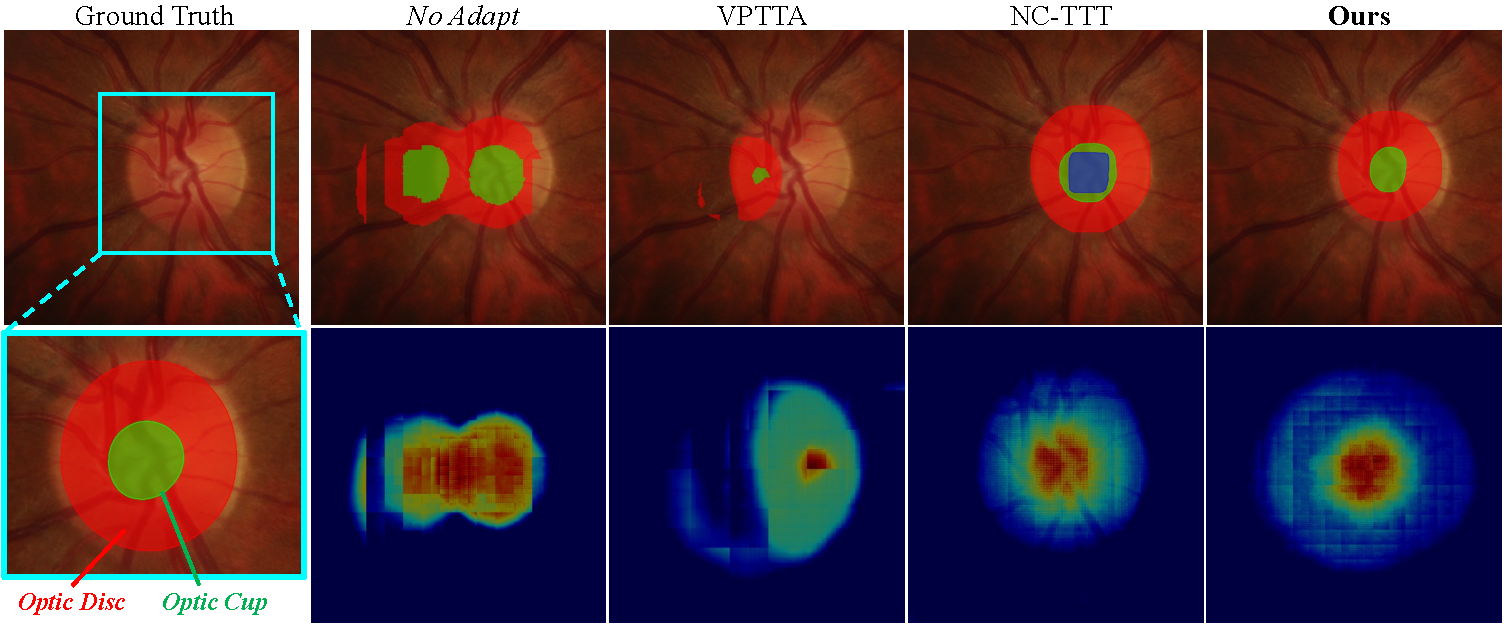
\includegraphics[width=0.999\linewidth]{Figures/visual_compare.pdf}
    % \vspace{-10pt}
    \caption{Visualization comparison of segmentation results and Grad-CAM outputs from the final layer of the backbone network for the \textit{No Adapt} baseline, VPTTA~\cite{chen2024each}, NC-TTT~\cite{osowiechi2024nc}, and our proposed method on retinal fundus images. Additional visual comparisons are provided in the supplementary material.}
     \vspace{-0.5cm}
    \label{fig:visual}
\end{figure}
\section{Analysis}

\begin{table}[htb!]
% \vspace{-9pt}
\setlength{\tabcolsep}{6pt}
\centering
  \caption{Ablation study in the retinal fundus segmentation. Details of the experiment can be found in Sec~\ref{sec:abl_ue}.}
  \vspace{-0.3cm}
  \begin{adjustbox}{width=0.999\linewidth}
    \begin{tabular}{c|ccccc|c}
\hlineB{3}
\multirow{2}{*}{Methods}     & Site A & Site B & Site C & Site D & Site E & Average \\ \cline{2-7}
& \multicolumn{6}{c}{\textbf{Dice Score Metric $\uparrow$ (DSC, mean$\pm$std )}} \\ \hline \hline

\textit{No Adapt} & 65.60\small{$\pm$5.78} & 74.65\small{$\pm$4.88} & 63.15\small{$\pm$7.30} & 68.11\small{$\pm$5.49} & 75.34\small{$\pm$1.01} & 69.37\\ \hline

\textit{w/o $\mathcal{U}$}      &  77.09\small{$\pm$1.90}      & 83.24\small{$\pm$2.01}       &  80.50\small{$\pm$1.44}      &  78.32\small{$\pm$1.55}      &    83.18\small{$\pm$2.18}    &  80.47       \\
\textit{w/o priors} &   79.51\small{$\pm$0.80}     & 79.36\small{$\pm$1.13}       &  77.40\small{$\pm$1.89}      &    77.29\small{$\pm$1.77}    &  80.00\small{$\pm$1.93}      &    78.71     \\
\hline
Ours &  82.53\small{$\pm$1.52} &  88.98\small{$\pm$0.89}      &  88.73\small{$\pm$0.70}      &  90.25\small{$\pm$1.33}      &   91.83\small{$\pm$0.71}     &   \textbf{88.46}    \\
\hlineB{3}
\end{tabular}
  \end{adjustbox}
  \label{tab:tabel_abl1}
\end{table}

% To assess the effectiveness of the universe embeddings, multi-graph matching, and the entire test-time paradigm, we conducted a series of ablation experiments on the retinal fundus datasets. The experimental settings remained consistent with those in Sec.~\ref{exp_setup}. For more detailed analysis, please refer to the supplementary material.

\subsection{Effectiveness of the Universe Embeddings}
\label{sec:abl_ue}
The universe embeddings $\mathcal{U}$ play a crucial role in incorporating morphological priors from medical images, resulting in an assignment matrix that projects each node to the \textit{universe of nodes}. To validate the effectiveness during the TTA, we conducted the following experiments: (1) Without universe embeddings (denoted as \textit{w/o $\mathcal{U}$}), the universe matching assignment matrix $\bold{U}$ is initialized following the setting in \cite{wang2020graduated} (i.e. $\bold{U}=1/d+10^{-3}z$, where $z\sim N(0,1)$), leading to random matching between the nodes and the universe; (2) Without morphological priors but with $\mathcal{U}$ (denoted as \textit{w/o priors}). As shown in Table~\ref{tab:tabel_abl1}, the performance in (1) is slightly better than in (2) by 1.76\% in terms of DSC on average. However, when using the pre-trained $\mathcal{U}$ derived from the source model, the segmentation results show a significant improvement. This highlights the effectiveness of the pre-trained morphological priors embedded in $\mathcal{U}$ for medical imaging tasks.

\begin{figure}[!t]
    \centering
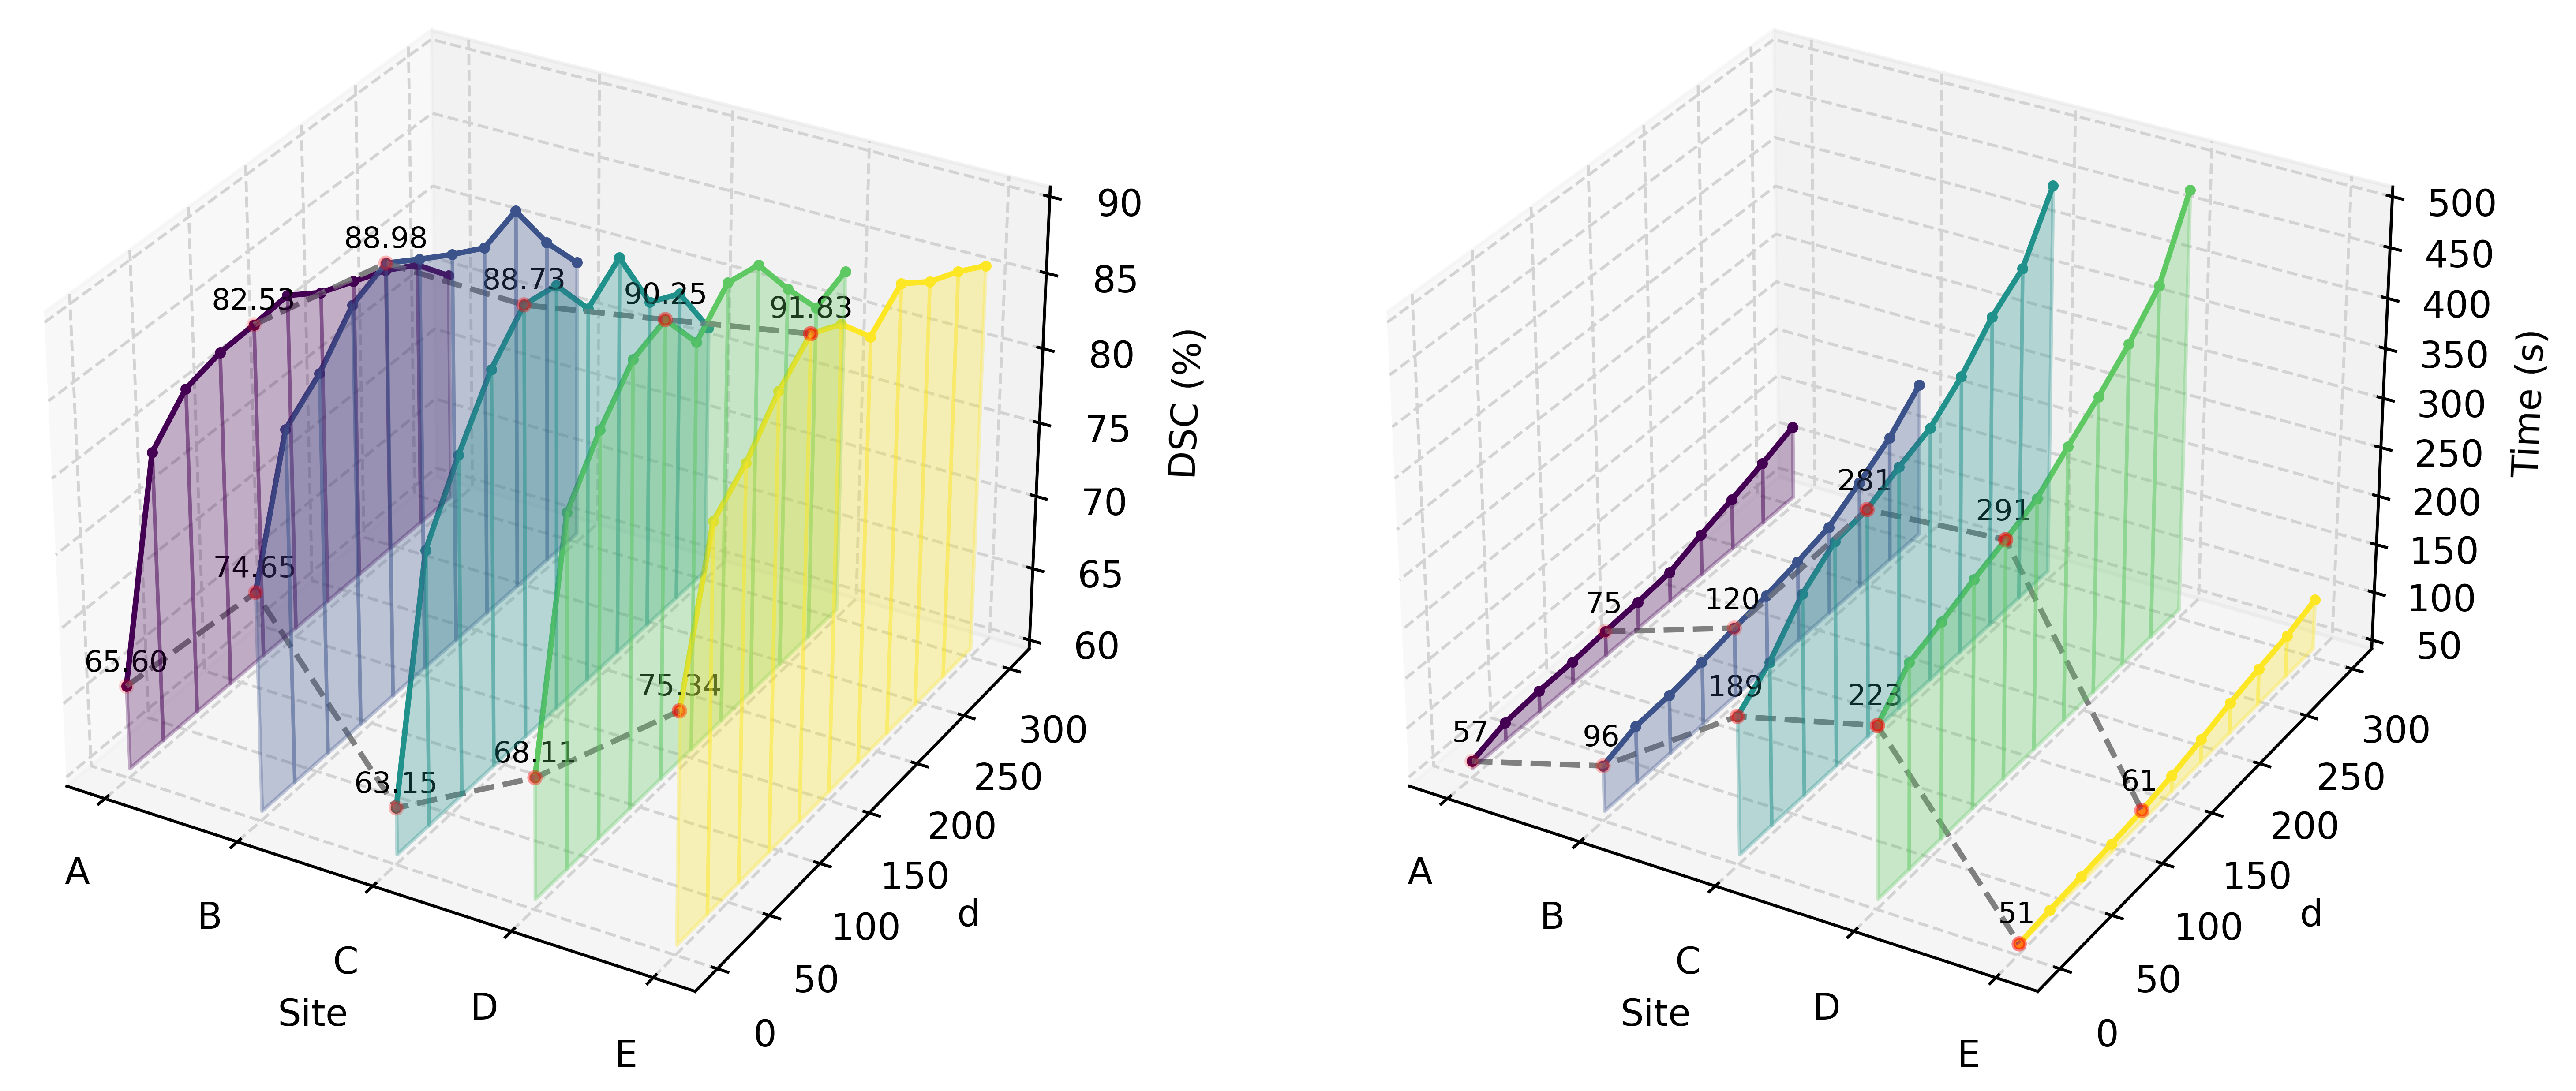
\includegraphics[width=0.999\linewidth]{Figures/comparison_dsc_time_labeled.png}
    % \vspace{-10pt}
    \caption{The performance of DSC (\%) and inference time (s) with different universe sizes $d$ are shown, with the experimental setup identical to that in Table~\ref{tab:tabel_fundus}. The first curve represents the \textit{No Adapt} baseline ($d = 0$), while the subsequent curve corresponds to the results obtained with a universe size of $ d = 120$.}
     \vspace{-0.5cm}
    \label{fig:universe_d}
\end{figure}

\vspace{-5pt}
\subsection{Effectiveness of the Universe Size}
The universe size $d$ directly impacts both the matching accuracy and computational efficiency, and its selection depends on the number of sampled nodes. Previous works~\cite{bernard2019hippi,wang2020graduated,nurlanov2023universe}, ensured that the $d$ matched the number of nodes in each graph by labeling an equal number of keypoints. In our experiments, $d$ is determined by the spatially-uniform sampling described in Sec~\ref{sec:graph_generation}, and we empirically set $d = 100\times (n+1) s^{-1}$, where $s$ is the sampling step and $n$ is the number of segmentation categories required for the task. We evaluated several $d$, with the results shown in Fig.~\ref{fig:universe_d}. We observe that excessively small or large step sizes—resulting in too many or too few sampled nodes—negatively impact both training speed and performance. However, when $d$ is within a reasonable range (in this experiment, $s \in[2, 10]$ i.e. $d \in [30, 150]$.), the model maintains good scalability and performance.

\begin{table}[htb!]
\vspace{-9pt}
\setlength{\tabcolsep}{8pt}
\centering
  \caption{Comparison of common variables and performance between pairwise matching and multi-matching, using the same experimental setup as in Table~\ref{tab:tabel_fundus}. Both methods follow the graph construction in Sec.~\ref{sec:graph_generation}.}
  \vspace{-0.3cm}
  \begin{adjustbox}{width=0.979\linewidth}
    \begin{tabular}{r|cc|l}
\hlineB{3}
\multirow{2}{*}{param} & \multicolumn{2}{c|}{Site A-E Average}              & \multirow{2}{*}{description}      \\ \cline{2-3}
&Pairwise~\cite{wang2019learning}         & Multi-Matching (Ours) & \\ \hline \hline
lr                     & $10^{-3}$ & $10^{-3}$ & learning rate \\
batch & 4 & 4  & batch size in  inference  \\
$h$ & 256 & 256  & dimension of node feature\\
$\tau$  & 0.05   & 0.05  & regularization factor of Sinkhorn \\
\textit{Iter} & 20 & 20 & max iterations of Sinkhorn        \\
$d$    & -  & 120 & universe size \\ \hline
DSC $\uparrow$  &  84.63   &  \textbf{88.46}  & dice score metric (\%) \\
time $\downarrow$& 0.930 &  \textbf{0.392}   & inference time per image (s/img)  \\
Param $\downarrow$ & 1.071 & \textbf{0.658} & parameter count (M) \\
FLOPs $\downarrow$&  15.35  &  \textbf{4.255}  &   floating point operations per second (G)  \\ \hlineB{3}
\end{tabular}

  \end{adjustbox}
  \label{tab:tabel_abl_matching}
\end{table}
\vspace{-0.5cm}
\subsection{Multi-Matching vs. Pairwise Matching}
Compared to pairwise matching, multi-matching uses cycle-consistency for global optimization, which helps avoid local optima in pairwise. Moreover, joint optimization reduces the computational complexity of large-scale matching. By incorporating morphological consistency constraints, multi-matching exhibits greater robustness. To validate these claims, we conducted experiments comparing the two approaches. 
For the pairwise matching method, we adopted the benchmark approach~\cite{wang2019learning} and applied the same graph construction process as in multi-matching. The comparison results are presented in Table~\ref{tab:tabel_abl_matching}. It is evident that multi-matching outperforms pairwise matching in terms of DSC, inference time, parameters and FLOPs.
The inference time of multi-matching was reduced by approximately 57.85\% compared to pairwise matching, while segmentation accuracy improved by 3.83\% in DSC.
\section{Conclusion}
This paper presents a novel multi-matching framework for TTDG, which leverages universe embeddings to incorporate morphological priors from medical images while ensuring cycle-consistency, along with an unsupervised test-time paradigm that fully integrates these priors for efficient adaptation.
Extensive experiments, including comparisons and ablation studies demonstrate that our graph-matching-based approach achieves SOTA performance, outperforming entropy-based, template-based, batch normalization-based, and noise estimation-based methods across both multi-source and single-source domain generalization tasks. 



\newpage
\section*{Acknowledgements}

This work was supported in part by the National Natural Science Foundation of China (Grant No. 62306003), the Open Research Fund from Guangdong Laboratory of Artificial Intelligence and Digital Economy (SZ), under Grant No. GML-KF-24-29 and the Open Foundation of Jiangxi Provincial Key Laboratory of Image Processing and Pattern Recognition (ET202404437).
{
    \small
    \bibliographystyle{ieeenat_fullname}
    \bibliography{main}
    
}

\clearpage
\appendix
\setcounter{page}{1}
\maketitlesupplementary

\section{Implementation Details}
We follow prior studies\cite{coop, cocoop, prograd, kgcoop, maple, tcp, mma} and adopt a 16-shot learning setting across all experiments, except for the few-shot learning tasks. The ViT-B/16\cite{vit} variant of the CLIP model serves as the visual backbone for all experimental setups. Hand-crafted text prompts from prior methods\cite{clip, coop, tip-adapter} are utilized and described in detail in \cref{datasets}. Optimization is performed using the AdamW optimizer with an initial learning rate of 0.001. All our models are trained with mix-precision for speeding up. For the larger ImageNet dataset, we employ a batch size of 32, while a batch size of 4 is used for all other datasets. Training on ImageNet for the base-to-novel generalization task spans 5 epochs, whereas training on the remaining datasets is conducted over 10 epochs. For cross-dataset evaluation and domain generalization tasks, we perform training for a single epoch on ImageNet. In the few-shot learning tasks, training is carried out for 5 epochs on ImageNet and 50 epochs for other datasets. The average accuracy is reported over three independent runs, with all experiments executed on a single NVIDIA RTX 4090 GPU.

Representation tokens are initialized from a zero-mean Gaussian distribution with a standard deviation of 0.02. We set $J = 6$, integrating the representation tokens beginning at the 6-th transformer layer. The dimension of the representation space, $d_r$, is set to 2048 for EuroSAT and 512 for all other datasets. Note that since the $d_r$ setting for EuroSAT differs from other datasets, in the $d_r$ ablation experiments we fix $d_r$ for EuroSAT to 2048 while adjusting $d_r$ on the other datasets. The number of representation tokens, $K$, is configured to 5. The parameter $\alpha$ is fixed at 0.7, and the details regarding the configuration of $\lambda$ are provided in \cref{ablation_lambda}.



\section{Dataset Details}
Details of 14 datasets are shown in \cref{datasets}.


\section{Computational Cost}
Table \ref{computational_cost} summarizes the learnable parameters, training time per image, total training duration, inference speed (measured in frames per second, FPS, with a batch size of 100), and the final HM metric for each approach. Our proposed model, MMRL, demonstrates a compelling balance of computational efficiency and performance. The key observations are as follows:
\begin{itemize}
    \item Models incorporating multimodal interaction mechanisms (e.g., MaPLe, MMA, and MMRL) generally involve a higher parameter count compared to models without such mechanisms.
    \item Both MMRL and the prior MMA approach exhibit significantly faster training speed, thereby reducing overall computational costs. While MaPLe and PromptSRC achieve higher inference speeds, their training durations are relatively longer. Notably, MMRL offers faster inference compared to MMA and MetaPrompt.
    \item To assess the performance of MMRL under constrained computational resources, we reduced the dimensionality of the representation space from 512 to 32. In this configuration, MMRL achieves a parameter count comparable to that of MMA, while still significantly outperforming the previous state-of-the-art model.
\end{itemize}



\begin{table}[h]
\centering
\renewcommand\arraystretch{1.25}
\caption{All methods were trained on a single NVIDIA RTX 4090 GPU using the ImageNet dataset. Each model was implemented with publicly available code and default configurations as described in their respective papers \cite{maple, promptsrc, provp, metaprompt, tcp, mma}. `V-L' denotes vision-language interaction, indicating that efficient fine-tuning incorporates interactions between visual and textual modalities before prediction. `V, L' signifies separate fine-tuning of each modality without inter-modal interaction before prediction, while `L' refers to fine-tuning limited to the textual modality alone. `Train time' is reported as both time per image and the total duration for training the full dataset(16-shots), while `FPS (100 BS)' indicates frames per second with a batch size of 100 during inference.}
\label{computational_cost}
\resizebox{0.475\textwidth}{!}{
    \begin{tabular}{@{}l|ccccc|c@{}}
    \toprule
    \multirow{2}{*}{Method} & \multirow{2}{*}{Modality} & Params & Train time & Train time & FPS & \multirow{2}{*}{HM} \\
               &     & (learnable) & (ms/image) & (minute/all) & (100 BS) &       \\ \midrule
    MaPLe      & V-L & 3.555M      & 39.5       & 26.4         & 1757.6   & 78.55 \\
    PromptSRC  & V,L & 0.046M      & 40.0       & 106.8        & 1764.2   & 79.97 \\
    ProVP      & V   & 0.147M      & 4.4        & 107.2        & 928.9    & 78.76 \\
    MetaPrompt & V,L & 0.031M      & 30.7       & 32.8         & 659.8    & 79.09 \\
    TCP        & L   & 0.332M      & 5.3        & 17.7         & 950.6    & 79.51 \\
    MMA        & V-L & 0.675M      & 2.2        & 1.5          & 688.5    & 79.87 \\ \midrule
    MMRL       & V-L & 4.992M      & 5.3        & 3.6          & 762.4    & 81.20 \\
    MMRL*      & V-L & 0.689M      & 5.3        & 3.6          & 767.8    & 80.84 \\ \bottomrule
    \end{tabular}
}
\end{table}


\section{Ablation Analysis on $\lambda$}
As shown in \cref{ablation_lambda}, increasing the value of $\lambda$ generally improves performance, with the optimal or near-optimal results typically observed when $\lambda$ is set between 4 and 6 across most datasets. Notably, as $\lambda$ continues to increase, its impact on model performance within the same dataset diminishes, indicating reduced sensitivity to variations in $\lambda$. This trend suggests that the model becomes more robust and less reliant on precise tuning of $\lambda$ at higher values.


\begin{table*}[h]
\centering
\caption{Summary of the 14 datasets.}
\label{datasets}
\renewcommand\arraystretch{1.2}
\resizebox{1.0\textwidth}{!}{
    \begin{tabular}{@{}l|llllll@{}}
    \toprule
    Dataset      & Classes & Train  & Val    & Test   & Description                         & Prompt                                \\ \midrule
    ImageNet     & 1000    & 1.28M  & $\sim$ & 50000  & Recognition of generic objects      & ``a photo of a [CLASS].”              \\
    Caltech101   & 100     & 4128   & 1649   & 2465   & Recognition of generic objects      & ``a photo of a [CLASS].”              \\
    OxfordPets      & 37    & 2944   & 736    & 3669   & Fine-grained classification of pets                    & ``a photo of a [CLASS], a type of pet.”      \\
    StanfordCars & 196     & 6509   & 1635   & 8041   & Fine-grained classification of cars & ``a photo of a [CLASS].”              \\
    Flowers102      & 102   & 4093   & 1633   & 2463   & Fine-grained classification of flowers                 & ``a photo of a [CLASS], a type of flower.”   \\
    Food101         & 101   & 50500  & 20200  & 30300  & Fine-grained classification of foods                   & ``a photo of [CLASS], a type of food.”       \\
    FGVCAircraft    & 100   & 3334   & 3333   & 3333   & Fine-grained classification of aircrafts               & ``a photo of a [CLASS], a type of aircraft.” \\
    SUN397       & 397     & 15880  & 3970   & 19850  & Scene classification                & ``a photo of a [CLASS].”              \\
    DTD          & 47      & 2820   & 1128   & 1692   & Texture classification              & ``[CLASS] texture.”                   \\
    EuroSAT         & 10    & 13500  & 5400   & 8100   & Land use \& cover classification with satellite images & ``a centered satellite photo of [CLASS].”    \\
    UCF101       & 101     & 7639   & 1898   & 3783   & Action recognition                  & ``a photo of a person doing [CLASS].” \\ \midrule
    ImageNetV2   & 1,000   & $\sim$ & $\sim$ & 10,000 & New test data for ImageNet          & ``a photo of a [CLASS].”              \\
    ImageNet-Sketch & 1,000 & $\sim$ & $\sim$ & 50,889 & Sketch-style images of ImageNet classes                & ``a photo of a [CLASS].”                     \\
    ImageNet-A      & 200   & $\sim$ & $\sim$ & 7,500  & Natural adversarial examples of 200 ImageNet classes   & ``a photo of a [CLASS].”                     \\
    ImageNet-R   & 200     & $\sim$ & $\sim$ & 30,000 & Renditions of 200 ImageNet classes  & ``a photo of a [CLASS].”              \\ \bottomrule
    \end{tabular}
    }
\end{table*}


\begin{table*}[h]
\centering
\caption{Ablation on $\lambda$ across 11 datasets, with results evaluated using the harmonic mean (HM) metric.}
\label{ablation_lambda}
\renewcommand\arraystretch{1.2}
\resizebox{1.0\textwidth}{!}{
    \begin{tabular}{@{}c|ccccccccccc@{}}
    \toprule
    $\alpha$ & ImageNet       & Caltech101     & OxfordPets & StanfordCars & Flowers102 & Food101 & FGVCAircraft   & SUN397         & DTD            & EuroSAT & UCF101 \\ \midrule
    0.0  & 74.01 & 95.97 & 96.35          & 76.00          & 84.42          & 90.10          & 38.52 & 79.67 & 68.21 & 82.65          & 81.63          \\
    0.01 & 74.07 & 96.12 & 96.39          & 75.95          & 84.82          & 90.23          & 37.87 & 79.85 & 67.73 & \textbf{87.21} & 82.11          \\
    0.1  & 74.23 & 96.25 & 96.49          & 76.32          & 84.81          & 90.53          & 38.66 & 80.23 & 69.79 & 83.21          & 82.91          \\
    0.2  & 74.38 & 96.40 & \textbf{96.74} & 76.67          & 85.31          & 90.61          & 39.27 & 80.25 & 70.58 & 82.68          & 82.70          \\
    0.5      & \textbf{74.45} & \textbf{96.68} & 96.54      & 77.09        & 85.74      & 90.86   & 40.37          & 80.61          & 72.67          & 82.87   & 83.05  \\
    3.0  & 74.09 & 96.59 & 96.51          & 77.72          & 86.65          & 90.98          & 40.48 & 81.10 & 73.54 & 77.95          & \textbf{83.89} \\
    4.0  & 74.04 & 96.62 & 96.55          & 77.73          & \textbf{86.78} & 90.98          & 40.66 & 81.14 & 73.75 & 77.27          & 83.45          \\
    5.0  & 73.93 & 96.62 & 96.60          & 77.86          & 86.42          & \textbf{91.03} & 40.42 & 81.07 & 73.69 & 78.05          & 83.84          \\
    6.0      & 73.83          & 96.61          & 96.66      & 78.05        & 86.48      & 91.00   & \textbf{41.15} & \textbf{81.20} & \textbf{73.82} & 75.23   & 83.68  \\
    7.0  & 73.78 & 96.62 & 96.58          & \textbf{78.06} & 86.53          & 90.95          & 40.88 & 81.10 & 73.65 & 75.85          & 83.55          \\
    10.0 & 73.68 & 96.64 & 96.56          & 77.86          & 86.46          & 91.00          & 41.01 & 80.93 & 73.68 & 77.61          & 83.38          \\ \bottomrule
    \end{tabular}
}
\end{table*}

\begin{table}[t]
\small
\centering
\caption{Ablation on different regularization strategies.}
\label{ablation_regularization}
\begin{tabular}{@{}c|ccc@{}}
\toprule
Regularization & Base           & Novel          & HM             \\ \midrule
\rowcolor[HTML]{EFEFEF} 
Cosine         & \textbf{85.68} & \textbf{77.16} & \textbf{81.20} \\
L1             & 85.46          & 76.03          & 80.47          \\
MSE             & 85.13          & 74.62          & 79.53          \\ \bottomrule
\end{tabular}
\end{table}

\section{Ablation Analysis on Regularization Strategies}
We investigate the impact of various regularization strategies aimed at maximizing the similarity between class token features and frozen CLIP features to retain pre-trained knowledge. The results, summarized in \cref{ablation_regularization}, indicate that cosine regularization achieves the best performance. In contrast, both L1 and MSE losses lead to performance degradation, with MSE causing a significant decline. This result can be attributed to the more relaxed and flexible constraints of cosine regularization, enabling the class token to preserve generalizability while effectively capturing task-specific knowledge.






\section{Few-Shot Learning}
\cref{few_shot1,few_shot2} provide detailed comparisons of MMRL and prior state-of-the-art methods on few-shot learning across 11 datasets. MMRL achieves the highest average performance across all shots. Note that the MMA results are reproduced from the open-source code, as the original paper does not report results for this experiment.







\begin{table*}[t]
\small
\centering
\caption{Comparison of MMRL with previous state-of-the-art methods on few-shot learning across 11 datasets.}
\label{few_shot1}
\setlength{\tabcolsep}{15pt}{
\resizebox{0.9\textwidth}{!}{
    \begin{tabular}{@{}ll|ccccc}
    \toprule
    \textbf{Dataset} &
      \textbf{Method} &
      \textbf{1 shot} &
      \textbf{2 shots} &
      \textbf{4 shots} &
      \textbf{8 shots} &
      \textbf{16 shots} \\ \midrule
     &
      Linear probe CLIP &
      45.83 &
      57.98 &
      68.01 &
      74.47 &
      78.79 \\
     &
      CoOp &
      67.56 &
      70.65 &
      74.02 &
      76.98 &
      79.89 \\
     &
      CoCoOp &
      66.79 &
      67.65 &
      71.21 &
      72.96 &
      74.90 \\
     &
      MaPLe &
      69.27 &
      72.58 &
      75.37 &
      78.89 &
      81.79 \\
     &
      PromptSRC &
      72.32 &
      75.29 &
      78.35 &
      80.69 &
      82.87 \\
     &
      MMA &
      69.28 &
      72.08 &
      76.38 &
      79.57 &
      82.76 \\
    \multirow{-7}{*}{Average} &
      \cellcolor[HTML]{E8E8E8}$\text{MMRL}_{\text{ (Ours)}}$ &
      \cellcolor[HTML]{E8E8E8}\textbf{72.67} &
      \cellcolor[HTML]{E8E8E8}\textbf{75.90} &
      \cellcolor[HTML]{E8E8E8}\textbf{79.20} &
      \cellcolor[HTML]{E8E8E8}\textbf{81.47} &
      \cellcolor[HTML]{E8E8E8}\textbf{84.34} \\ \midrule
     &
      Linear probe CLIP &
      32.13 &
      44.88 &
      54.85 &
      62.23 &
      67.31 \\
     &
      CoOp &
      66.33 &
      67.07 &
      68.73 &
      70.63 &
      71.87 \\
     &
      CoCoOp &
      69.43 &
      69.78 &
      70.39 &
      70.63 &
      70.83 \\
     &
      MaPLe &
      62.67 &
      65.10 &
      67.70 &
      70.30 &
      72.33 \\
     &
      PromptSRC &
      68.13 &
      69.77 &
      71.07 &
      \textbf{72.33} &
      73.17 \\
     &
      MMA &
      \textbf{69.17} &
      \textbf{70.37} &
      71.00 &
      71.77 &
      73.13 \\
    \multirow{-7}{*}{ImageNet} &
      \cellcolor[HTML]{E8E8E8}$\text{MMRL}_{\text{ (Ours)}}$ &
      \cellcolor[HTML]{E8E8E8}69.00 &
      \cellcolor[HTML]{E8E8E8}70.30 &
      \cellcolor[HTML]{E8E8E8}\textbf{71.40} &
      \cellcolor[HTML]{E8E8E8}\textbf{72.33} &
      \cellcolor[HTML]{E8E8E8}\textbf{73.40} \\ \midrule
     &
      Linear probe CLIP &
      79.88 &
      89.01 &
      92.05 &
      93.41 &
      95.43 \\
     &
      CoOp &
      92.60 &
      93.07 &
      94.40 &
      94.37 &
      95.57 \\
     &
      CoCoOp &
      93.83 &
      94.82 &
      94.98 &
      95.04 &
      95.16 \\
     &
      MaPLe &
      92.57 &
      93.97 &
      94.43 &
      95.20 &
      96.00 \\
     &
      PromptSRC &
      93.67 &
      94.53 &
      95.27 &
      95.67 &
      96.07 \\
     &
      MMA &
      92.90 &
      94.00 &
      94.33 &
      95.37 &
      96.33 \\
    \multirow{-7}{*}{Caltech101} &
      \cellcolor[HTML]{E8E8E8}$\text{MMRL}_{\text{ (Ours)}}$ &
      \cellcolor[HTML]{E8E8E8}\textbf{94.17} &
      \cellcolor[HTML]{E8E8E8}\textbf{94.83} &
      \cellcolor[HTML]{E8E8E8}\textbf{96.03} &
      \cellcolor[HTML]{E8E8E8}\textbf{96.27} &
      \cellcolor[HTML]{E8E8E8}\textbf{97.13} \\ \midrule
     &
      Linear probe CLIP &
      44.06 &
      58.37 &
      71.17 &
      78.36 &
      85.34 \\
     &
      CoOp &
      90.37 &
      89.80 &
      92.57 &
      91.27 &
      91.87 \\
     &
      CoCoOp &
      91.27 &
      \textbf{92.64} &
      92.81 &
      93.45 &
      93.34 \\
     &
      MaPLe &
      89.10 &
      90.87 &
      91.90 &
      92.57 &
      92.83 \\
     &
      PromptSRC &
      \textbf{92.00} &
      92.50 &
      \textbf{93.43} &
      \textbf{93.50} &
      93.67 \\
     &
      MMA &
      91.23 &
      91.97 &
      92.23 &
      92.77 &
      93.23 \\
    \multirow{-7}{*}{OxfordPets} &
      \cellcolor[HTML]{E8E8E8}$\text{MMRL}_{\text{ (Ours)}}$ &
      \cellcolor[HTML]{E8E8E8}90.87 &
      \cellcolor[HTML]{E8E8E8}91.57 &
      \cellcolor[HTML]{E8E8E8}92.57 &
      \cellcolor[HTML]{E8E8E8}93.03 &
      \cellcolor[HTML]{E8E8E8}\textbf{93.83} \\ \midrule
     &
      Linear probe CLIP &
      35.66 &
      50.28 &
      63.38 &
      73.67 &
      80.44 \\
     &
      CoOp &
      67.43 &
      70.50 &
      74.47 &
      79.30 &
      83.07 \\
     &
      CoCoOp &
      67.22 &
      68.37 &
      69.39 &
      70.44 &
      71.57 \\
     &
      MaPLe &
      66.60 &
      71.60 &
      75.30 &
      79.47 &
      83.57 \\
     &
      PromptSRC &
      \textbf{69.40} &
      \textbf{73.40} &
      77.13 &
      80.97 &
      83.83 \\
     &
      MMA &
      67.87 &
      71.77 &
      76.50 &
      81.40 &
      85.70 \\
    \multirow{-7}{*}{StanfordCars} &
      \cellcolor[HTML]{E8E8E8}$\text{MMRL}_{\text{ (Ours)}}$ &
      \cellcolor[HTML]{E8E8E8}68.70 &
      \cellcolor[HTML]{E8E8E8}72.93 &
      \cellcolor[HTML]{E8E8E8}\textbf{78.17} &
      \cellcolor[HTML]{E8E8E8}\textbf{82.57} &
      \cellcolor[HTML]{E8E8E8}\textbf{86.43} \\ \midrule
     &
      Linear probe CLIP &
      69.74 &
      85.07 &
      92.02 &
      96.10 &
      97.37 \\
     &
      CoOp &
      77.53 &
      87.33 &
      92.17 &
      94.97 &
      97.07 \\
     &
      CoCoOp &
      72.08 &
      75.79 &
      78.40 &
      84.30 &
      87.84 \\
     &
      MaPLe &
      83.30 &
      88.93 &
      92.67 &
      95.80 &
      97.00 \\
     &
      PromptSRC &
      85.93 &
      91.17 &
      93.87 &
      96.27 &
      97.60 \\
     &
      MMA &
      83.60 &
      90.30 &
      93.00 &
      95.97 &
      97.97 \\
    \multirow{-7}{*}{Flowers102} &
      \cellcolor[HTML]{E8E8E8}$\text{MMRL}_{\text{ (Ours)}}$ &
      \cellcolor[HTML]{E8E8E8}\textbf{85.97} &
      \cellcolor[HTML]{E8E8E8}\textbf{91.20} &
      \cellcolor[HTML]{E8E8E8}\textbf{94.60} &
      \cellcolor[HTML]{E8E8E8}\textbf{96.60} &
      \cellcolor[HTML]{E8E8E8}\textbf{98.40} \\ \bottomrule
    \end{tabular}
    }
    }
\end{table*}


\begin{table*}[t]
\small
\centering
\caption{Comparison of MMRL with previous state-of-the-art methods on few-shot learning across 11 datasets.}
\label{few_shot2}
\setlength{\tabcolsep}{15pt}{
\resizebox{0.9\textwidth}{!}{
    \begin{tabular}{@{}ll|ccccc}
    \toprule
    \textbf{Dataset} &
      \textbf{Method} &
      \textbf{1 shot} &
      \textbf{2 shots} &
      \textbf{4 shots} &
      \textbf{8 shots} &
      \textbf{16 shots} \\ \midrule
     &
      Linear probe CLIP &
      43.96 &
      61.51 &
      73.19 &
      79.79 &
      82.90 \\
     &
      CoOp &
      84.33 &
      84.40 &
      84.47 &
      82.67 &
      84.20 \\
     &
      CoCoOp &
      \textbf{85.65} &
      \textbf{86.22} &
      \textbf{86.88} &
      \textbf{86.97} &
      87.25 \\
     &
      MaPLe &
      80.50 &
      81.47 &
      81.77 &
      83.60 &
      85.33 \\
     &
      PromptSRC &
      84.87 &
      85.70 &
      86.17 &
      86.90 &
      \textbf{87.50} \\
     &
      MMA &
      83.03 &
      82.50 &
      82.13 &
      83.00 &
      84.57 \\
    \multirow{-7}{*}{Food101} &
      \cellcolor[HTML]{E8E8E8}$\text{MMRL}_{\text{ (Ours)}}$ &
      \cellcolor[HTML]{E8E8E8}84.87 &
      \cellcolor[HTML]{E8E8E8}85.53 &
      \cellcolor[HTML]{E8E8E8}85.77 &
      \cellcolor[HTML]{E8E8E8}86.33 &
      \cellcolor[HTML]{E8E8E8}87.03 \\ \midrule
     &
      Linear probe CLIP &
      19.61 &
      26.41 &
      32.33 &
      39.35 &
      45.36 \\
     &
      CoOp &
      21.37 &
      26.20 &
      30.83 &
      39.00 &
      43.40 \\
     &
      CoCoOp &
      12.68 &
      15.06 &
      24.79 &
      26.61 &
      31.21 \\
     &
      MaPLe &
      26.73 &
      30.90 &
      34.87 &
      42.00 &
      48.40 \\
     &
      PromptSRC &
      27.67 &
      31.70 &
      37.47 &
      43.27 &
      50.83 \\
     &
      MMA &
      \textbf{28.73} &
      31.90 &
      37.57 &
      44.83 &
      52.70 \\
    \multirow{-7}{*}{FGVCAircraft} &
      \cellcolor[HTML]{E8E8E8}$\text{MMRL}_{\text{ (Ours)}}$ &
      \cellcolor[HTML]{E8E8E8}28.53 &
      \cellcolor[HTML]{E8E8E8}\textbf{34.23} &
      \cellcolor[HTML]{E8E8E8}\textbf{40.47} &
      \cellcolor[HTML]{E8E8E8}\textbf{48.07} &
      \cellcolor[HTML]{E8E8E8}\textbf{57.60} \\ \midrule
     &
      Linear probe CLIP &
      41.58 &
      53.70 &
      63.00 &
      69.08 &
      73.28 \\
     &
      CoOp &
      66.77 &
      66.53 &
      69.97 &
      71.53 &
      74.67 \\
     &
      CoCoOp &
      68.33 &
      69.03 &
      70.21 &
      70.84 &
      72.15 \\
     &
      MaPLe &
      64.77 &
      67.10 &
      70.67 &
      73.23 &
      75.53 \\
     &
      PromptSRC &
      \textbf{69.67} &
      \textbf{71.60} &
      \textbf{74.00} &
      75.73 &
      77.23 \\
     &
      MMA &
      64.00 &
      67.17 &
      69.97 &
      72.30 &
      74.63 \\
    \multirow{-7}{*}{SUN397} &
      \cellcolor[HTML]{E8E8E8}$\text{MMRL}_{\text{ (Ours)}}$ &
      \cellcolor[HTML]{E8E8E8}68.90 &
      \cellcolor[HTML]{E8E8E8}71.53 &
      \cellcolor[HTML]{E8E8E8}73.93 &
      \cellcolor[HTML]{E8E8E8}\textbf{76.00} &
      \cellcolor[HTML]{E8E8E8}\textbf{77.70} \\ \midrule
     &
      Linear probe CLIP &
      34.59 &
      40.76 &
      55.71 &
      63.46 &
      69.96 \\
     &
      CoOp &
      50.23 &
      53.60 &
      58.70 &
      64.77 &
      69.87 \\
     &
      CoCoOp &
      48.54 &
      52.17 &
      55.04 &
      58.89 &
      63.04 \\
     &
      MaPLe &
      52.13 &
      55.50 &
      61.00 &
      66.50 &
      71.33 \\
     &
      PromptSRC &
      56.23 &
      59.97 &
      65.53 &
      69.87 &
      72.73 \\
     &
      MMA &
      52.27 &
      56.90 &
      63.93 &
      67.97 &
      73.47 \\
    \multirow{-7}{*}{DTD} &
      \cellcolor[HTML]{E8E8E8}$\text{MMRL}_{\text{ (Ours)}}$ &
      \cellcolor[HTML]{E8E8E8}\textbf{56.37} &
      \cellcolor[HTML]{E8E8E8}\textbf{61.37} &
      \cellcolor[HTML]{E8E8E8}\textbf{67.87} &
      \cellcolor[HTML]{E8E8E8}\textbf{71.60} &
      \cellcolor[HTML]{E8E8E8}\textbf{75.30} \\ \midrule
     &
      Linear probe CLIP &
      49.23 &
      61.98 &
      77.09 &
      84.43 &
      87.21 \\
     &
      CoOp &
      54.93 &
      65.17 &
      70.80 &
      78.07 &
      84.93 \\
     &
      CoCoOp &
      55.33 &
      46.74 &
      65.56 &
      68.21 &
      73.32 \\
     &
      MaPLe &
      71.80 &
      78.30 &
      84.50 &
      87.73 &
      92.33 \\
     &
      PromptSRC &
      73.13 &
      79.37 &
      86.30 &
      \textbf{88.80} &
      92.43 \\
     &
      MMA &
      55.07 &
      59.80 &
      79.40 &
      86.47 &
      92.37 \\
    \multirow{-7}{*}{EuroSAT} &
      \cellcolor[HTML]{E8E8E8}$\text{MMRL}_{\text{ (Ours)}}$ &
      \cellcolor[HTML]{E8E8E8}\textbf{76.00} &
      \cellcolor[HTML]{E8E8E8}\textbf{82.87} &
      \cellcolor[HTML]{E8E8E8}\textbf{87.67} &
      \cellcolor[HTML]{E8E8E8}88.73 &
      \cellcolor[HTML]{E8E8E8}\textbf{93.37} \\ \midrule
     &
      Linear probe CLIP &
      53.66 &
      65.78 &
      73.28 &
      79.34 &
      82.11 \\
     &
      CoOp &
      71.23 &
      73.43 &
      77.10 &
      80.20 &
      82.23 \\
     &
      CoCoOp &
      70.30 &
      73.51 &
      74.82 &
      77.14 &
      78.14 \\
     &
      MaPLe &
      71.83 &
      74.60 &
      78.47 &
      81.37 &
      85.03 \\
     &
      PromptSRC &
      74.80 &
      \textbf{78.50} &
      81.57 &
      84.30 &
      86.47 \\
     &
      MMA &
      74.17 &
      76.17 &
      80.10 &
      83.43 &
      86.30 \\
    \multirow{-7}{*}{UCF101} &
      \cellcolor[HTML]{E8E8E8}$\text{MMRL}_{\text{ (Ours)}}$ &
      \cellcolor[HTML]{E8E8E8}\textbf{75.97} &
      \cellcolor[HTML]{E8E8E8}\textbf{78.50} &
      \cellcolor[HTML]{E8E8E8}\textbf{82.67} &
      \cellcolor[HTML]{E8E8E8}\textbf{84.67} &
      \cellcolor[HTML]{E8E8E8}\textbf{87.60} \\ \bottomrule
    \end{tabular}
    }
    }
\end{table*}




% WARNING: do not forget to delete the supplementary pages from your submission 
% \clearpage
\appendix
\setcounter{page}{1}
\maketitlesupplementary

\section{Implementation Details}
We follow prior studies\cite{coop, cocoop, prograd, kgcoop, maple, tcp, mma} and adopt a 16-shot learning setting across all experiments, except for the few-shot learning tasks. The ViT-B/16\cite{vit} variant of the CLIP model serves as the visual backbone for all experimental setups. Hand-crafted text prompts from prior methods\cite{clip, coop, tip-adapter} are utilized and described in detail in \cref{datasets}. Optimization is performed using the AdamW optimizer with an initial learning rate of 0.001. All our models are trained with mix-precision for speeding up. For the larger ImageNet dataset, we employ a batch size of 32, while a batch size of 4 is used for all other datasets. Training on ImageNet for the base-to-novel generalization task spans 5 epochs, whereas training on the remaining datasets is conducted over 10 epochs. For cross-dataset evaluation and domain generalization tasks, we perform training for a single epoch on ImageNet. In the few-shot learning tasks, training is carried out for 5 epochs on ImageNet and 50 epochs for other datasets. The average accuracy is reported over three independent runs, with all experiments executed on a single NVIDIA RTX 4090 GPU.

Representation tokens are initialized from a zero-mean Gaussian distribution with a standard deviation of 0.02. We set $J = 6$, integrating the representation tokens beginning at the 6-th transformer layer. The dimension of the representation space, $d_r$, is set to 2048 for EuroSAT and 512 for all other datasets. Note that since the $d_r$ setting for EuroSAT differs from other datasets, in the $d_r$ ablation experiments we fix $d_r$ for EuroSAT to 2048 while adjusting $d_r$ on the other datasets. The number of representation tokens, $K$, is configured to 5. The parameter $\alpha$ is fixed at 0.7, and the details regarding the configuration of $\lambda$ are provided in \cref{ablation_lambda}.



\section{Dataset Details}
Details of 14 datasets are shown in \cref{datasets}.


\section{Computational Cost}
Table \ref{computational_cost} summarizes the learnable parameters, training time per image, total training duration, inference speed (measured in frames per second, FPS, with a batch size of 100), and the final HM metric for each approach. Our proposed model, MMRL, demonstrates a compelling balance of computational efficiency and performance. The key observations are as follows:
\begin{itemize}
    \item Models incorporating multimodal interaction mechanisms (e.g., MaPLe, MMA, and MMRL) generally involve a higher parameter count compared to models without such mechanisms.
    \item Both MMRL and the prior MMA approach exhibit significantly faster training speed, thereby reducing overall computational costs. While MaPLe and PromptSRC achieve higher inference speeds, their training durations are relatively longer. Notably, MMRL offers faster inference compared to MMA and MetaPrompt.
    \item To assess the performance of MMRL under constrained computational resources, we reduced the dimensionality of the representation space from 512 to 32. In this configuration, MMRL achieves a parameter count comparable to that of MMA, while still significantly outperforming the previous state-of-the-art model.
\end{itemize}



\begin{table}[h]
\centering
\renewcommand\arraystretch{1.25}
\caption{All methods were trained on a single NVIDIA RTX 4090 GPU using the ImageNet dataset. Each model was implemented with publicly available code and default configurations as described in their respective papers \cite{maple, promptsrc, provp, metaprompt, tcp, mma}. `V-L' denotes vision-language interaction, indicating that efficient fine-tuning incorporates interactions between visual and textual modalities before prediction. `V, L' signifies separate fine-tuning of each modality without inter-modal interaction before prediction, while `L' refers to fine-tuning limited to the textual modality alone. `Train time' is reported as both time per image and the total duration for training the full dataset(16-shots), while `FPS (100 BS)' indicates frames per second with a batch size of 100 during inference.}
\label{computational_cost}
\resizebox{0.475\textwidth}{!}{
    \begin{tabular}{@{}l|ccccc|c@{}}
    \toprule
    \multirow{2}{*}{Method} & \multirow{2}{*}{Modality} & Params & Train time & Train time & FPS & \multirow{2}{*}{HM} \\
               &     & (learnable) & (ms/image) & (minute/all) & (100 BS) &       \\ \midrule
    MaPLe      & V-L & 3.555M      & 39.5       & 26.4         & 1757.6   & 78.55 \\
    PromptSRC  & V,L & 0.046M      & 40.0       & 106.8        & 1764.2   & 79.97 \\
    ProVP      & V   & 0.147M      & 4.4        & 107.2        & 928.9    & 78.76 \\
    MetaPrompt & V,L & 0.031M      & 30.7       & 32.8         & 659.8    & 79.09 \\
    TCP        & L   & 0.332M      & 5.3        & 17.7         & 950.6    & 79.51 \\
    MMA        & V-L & 0.675M      & 2.2        & 1.5          & 688.5    & 79.87 \\ \midrule
    MMRL       & V-L & 4.992M      & 5.3        & 3.6          & 762.4    & 81.20 \\
    MMRL*      & V-L & 0.689M      & 5.3        & 3.6          & 767.8    & 80.84 \\ \bottomrule
    \end{tabular}
}
\end{table}


\section{Ablation Analysis on $\lambda$}
As shown in \cref{ablation_lambda}, increasing the value of $\lambda$ generally improves performance, with the optimal or near-optimal results typically observed when $\lambda$ is set between 4 and 6 across most datasets. Notably, as $\lambda$ continues to increase, its impact on model performance within the same dataset diminishes, indicating reduced sensitivity to variations in $\lambda$. This trend suggests that the model becomes more robust and less reliant on precise tuning of $\lambda$ at higher values.


\begin{table*}[h]
\centering
\caption{Summary of the 14 datasets.}
\label{datasets}
\renewcommand\arraystretch{1.2}
\resizebox{1.0\textwidth}{!}{
    \begin{tabular}{@{}l|llllll@{}}
    \toprule
    Dataset      & Classes & Train  & Val    & Test   & Description                         & Prompt                                \\ \midrule
    ImageNet     & 1000    & 1.28M  & $\sim$ & 50000  & Recognition of generic objects      & ``a photo of a [CLASS].”              \\
    Caltech101   & 100     & 4128   & 1649   & 2465   & Recognition of generic objects      & ``a photo of a [CLASS].”              \\
    OxfordPets      & 37    & 2944   & 736    & 3669   & Fine-grained classification of pets                    & ``a photo of a [CLASS], a type of pet.”      \\
    StanfordCars & 196     & 6509   & 1635   & 8041   & Fine-grained classification of cars & ``a photo of a [CLASS].”              \\
    Flowers102      & 102   & 4093   & 1633   & 2463   & Fine-grained classification of flowers                 & ``a photo of a [CLASS], a type of flower.”   \\
    Food101         & 101   & 50500  & 20200  & 30300  & Fine-grained classification of foods                   & ``a photo of [CLASS], a type of food.”       \\
    FGVCAircraft    & 100   & 3334   & 3333   & 3333   & Fine-grained classification of aircrafts               & ``a photo of a [CLASS], a type of aircraft.” \\
    SUN397       & 397     & 15880  & 3970   & 19850  & Scene classification                & ``a photo of a [CLASS].”              \\
    DTD          & 47      & 2820   & 1128   & 1692   & Texture classification              & ``[CLASS] texture.”                   \\
    EuroSAT         & 10    & 13500  & 5400   & 8100   & Land use \& cover classification with satellite images & ``a centered satellite photo of [CLASS].”    \\
    UCF101       & 101     & 7639   & 1898   & 3783   & Action recognition                  & ``a photo of a person doing [CLASS].” \\ \midrule
    ImageNetV2   & 1,000   & $\sim$ & $\sim$ & 10,000 & New test data for ImageNet          & ``a photo of a [CLASS].”              \\
    ImageNet-Sketch & 1,000 & $\sim$ & $\sim$ & 50,889 & Sketch-style images of ImageNet classes                & ``a photo of a [CLASS].”                     \\
    ImageNet-A      & 200   & $\sim$ & $\sim$ & 7,500  & Natural adversarial examples of 200 ImageNet classes   & ``a photo of a [CLASS].”                     \\
    ImageNet-R   & 200     & $\sim$ & $\sim$ & 30,000 & Renditions of 200 ImageNet classes  & ``a photo of a [CLASS].”              \\ \bottomrule
    \end{tabular}
    }
\end{table*}


\begin{table*}[h]
\centering
\caption{Ablation on $\lambda$ across 11 datasets, with results evaluated using the harmonic mean (HM) metric.}
\label{ablation_lambda}
\renewcommand\arraystretch{1.2}
\resizebox{1.0\textwidth}{!}{
    \begin{tabular}{@{}c|ccccccccccc@{}}
    \toprule
    $\alpha$ & ImageNet       & Caltech101     & OxfordPets & StanfordCars & Flowers102 & Food101 & FGVCAircraft   & SUN397         & DTD            & EuroSAT & UCF101 \\ \midrule
    0.0  & 74.01 & 95.97 & 96.35          & 76.00          & 84.42          & 90.10          & 38.52 & 79.67 & 68.21 & 82.65          & 81.63          \\
    0.01 & 74.07 & 96.12 & 96.39          & 75.95          & 84.82          & 90.23          & 37.87 & 79.85 & 67.73 & \textbf{87.21} & 82.11          \\
    0.1  & 74.23 & 96.25 & 96.49          & 76.32          & 84.81          & 90.53          & 38.66 & 80.23 & 69.79 & 83.21          & 82.91          \\
    0.2  & 74.38 & 96.40 & \textbf{96.74} & 76.67          & 85.31          & 90.61          & 39.27 & 80.25 & 70.58 & 82.68          & 82.70          \\
    0.5      & \textbf{74.45} & \textbf{96.68} & 96.54      & 77.09        & 85.74      & 90.86   & 40.37          & 80.61          & 72.67          & 82.87   & 83.05  \\
    3.0  & 74.09 & 96.59 & 96.51          & 77.72          & 86.65          & 90.98          & 40.48 & 81.10 & 73.54 & 77.95          & \textbf{83.89} \\
    4.0  & 74.04 & 96.62 & 96.55          & 77.73          & \textbf{86.78} & 90.98          & 40.66 & 81.14 & 73.75 & 77.27          & 83.45          \\
    5.0  & 73.93 & 96.62 & 96.60          & 77.86          & 86.42          & \textbf{91.03} & 40.42 & 81.07 & 73.69 & 78.05          & 83.84          \\
    6.0      & 73.83          & 96.61          & 96.66      & 78.05        & 86.48      & 91.00   & \textbf{41.15} & \textbf{81.20} & \textbf{73.82} & 75.23   & 83.68  \\
    7.0  & 73.78 & 96.62 & 96.58          & \textbf{78.06} & 86.53          & 90.95          & 40.88 & 81.10 & 73.65 & 75.85          & 83.55          \\
    10.0 & 73.68 & 96.64 & 96.56          & 77.86          & 86.46          & 91.00          & 41.01 & 80.93 & 73.68 & 77.61          & 83.38          \\ \bottomrule
    \end{tabular}
}
\end{table*}

\begin{table}[t]
\small
\centering
\caption{Ablation on different regularization strategies.}
\label{ablation_regularization}
\begin{tabular}{@{}c|ccc@{}}
\toprule
Regularization & Base           & Novel          & HM             \\ \midrule
\rowcolor[HTML]{EFEFEF} 
Cosine         & \textbf{85.68} & \textbf{77.16} & \textbf{81.20} \\
L1             & 85.46          & 76.03          & 80.47          \\
MSE             & 85.13          & 74.62          & 79.53          \\ \bottomrule
\end{tabular}
\end{table}

\section{Ablation Analysis on Regularization Strategies}
We investigate the impact of various regularization strategies aimed at maximizing the similarity between class token features and frozen CLIP features to retain pre-trained knowledge. The results, summarized in \cref{ablation_regularization}, indicate that cosine regularization achieves the best performance. In contrast, both L1 and MSE losses lead to performance degradation, with MSE causing a significant decline. This result can be attributed to the more relaxed and flexible constraints of cosine regularization, enabling the class token to preserve generalizability while effectively capturing task-specific knowledge.






\section{Few-Shot Learning}
\cref{few_shot1,few_shot2} provide detailed comparisons of MMRL and prior state-of-the-art methods on few-shot learning across 11 datasets. MMRL achieves the highest average performance across all shots. Note that the MMA results are reproduced from the open-source code, as the original paper does not report results for this experiment.







\begin{table*}[t]
\small
\centering
\caption{Comparison of MMRL with previous state-of-the-art methods on few-shot learning across 11 datasets.}
\label{few_shot1}
\setlength{\tabcolsep}{15pt}{
\resizebox{0.9\textwidth}{!}{
    \begin{tabular}{@{}ll|ccccc}
    \toprule
    \textbf{Dataset} &
      \textbf{Method} &
      \textbf{1 shot} &
      \textbf{2 shots} &
      \textbf{4 shots} &
      \textbf{8 shots} &
      \textbf{16 shots} \\ \midrule
     &
      Linear probe CLIP &
      45.83 &
      57.98 &
      68.01 &
      74.47 &
      78.79 \\
     &
      CoOp &
      67.56 &
      70.65 &
      74.02 &
      76.98 &
      79.89 \\
     &
      CoCoOp &
      66.79 &
      67.65 &
      71.21 &
      72.96 &
      74.90 \\
     &
      MaPLe &
      69.27 &
      72.58 &
      75.37 &
      78.89 &
      81.79 \\
     &
      PromptSRC &
      72.32 &
      75.29 &
      78.35 &
      80.69 &
      82.87 \\
     &
      MMA &
      69.28 &
      72.08 &
      76.38 &
      79.57 &
      82.76 \\
    \multirow{-7}{*}{Average} &
      \cellcolor[HTML]{E8E8E8}$\text{MMRL}_{\text{ (Ours)}}$ &
      \cellcolor[HTML]{E8E8E8}\textbf{72.67} &
      \cellcolor[HTML]{E8E8E8}\textbf{75.90} &
      \cellcolor[HTML]{E8E8E8}\textbf{79.20} &
      \cellcolor[HTML]{E8E8E8}\textbf{81.47} &
      \cellcolor[HTML]{E8E8E8}\textbf{84.34} \\ \midrule
     &
      Linear probe CLIP &
      32.13 &
      44.88 &
      54.85 &
      62.23 &
      67.31 \\
     &
      CoOp &
      66.33 &
      67.07 &
      68.73 &
      70.63 &
      71.87 \\
     &
      CoCoOp &
      69.43 &
      69.78 &
      70.39 &
      70.63 &
      70.83 \\
     &
      MaPLe &
      62.67 &
      65.10 &
      67.70 &
      70.30 &
      72.33 \\
     &
      PromptSRC &
      68.13 &
      69.77 &
      71.07 &
      \textbf{72.33} &
      73.17 \\
     &
      MMA &
      \textbf{69.17} &
      \textbf{70.37} &
      71.00 &
      71.77 &
      73.13 \\
    \multirow{-7}{*}{ImageNet} &
      \cellcolor[HTML]{E8E8E8}$\text{MMRL}_{\text{ (Ours)}}$ &
      \cellcolor[HTML]{E8E8E8}69.00 &
      \cellcolor[HTML]{E8E8E8}70.30 &
      \cellcolor[HTML]{E8E8E8}\textbf{71.40} &
      \cellcolor[HTML]{E8E8E8}\textbf{72.33} &
      \cellcolor[HTML]{E8E8E8}\textbf{73.40} \\ \midrule
     &
      Linear probe CLIP &
      79.88 &
      89.01 &
      92.05 &
      93.41 &
      95.43 \\
     &
      CoOp &
      92.60 &
      93.07 &
      94.40 &
      94.37 &
      95.57 \\
     &
      CoCoOp &
      93.83 &
      94.82 &
      94.98 &
      95.04 &
      95.16 \\
     &
      MaPLe &
      92.57 &
      93.97 &
      94.43 &
      95.20 &
      96.00 \\
     &
      PromptSRC &
      93.67 &
      94.53 &
      95.27 &
      95.67 &
      96.07 \\
     &
      MMA &
      92.90 &
      94.00 &
      94.33 &
      95.37 &
      96.33 \\
    \multirow{-7}{*}{Caltech101} &
      \cellcolor[HTML]{E8E8E8}$\text{MMRL}_{\text{ (Ours)}}$ &
      \cellcolor[HTML]{E8E8E8}\textbf{94.17} &
      \cellcolor[HTML]{E8E8E8}\textbf{94.83} &
      \cellcolor[HTML]{E8E8E8}\textbf{96.03} &
      \cellcolor[HTML]{E8E8E8}\textbf{96.27} &
      \cellcolor[HTML]{E8E8E8}\textbf{97.13} \\ \midrule
     &
      Linear probe CLIP &
      44.06 &
      58.37 &
      71.17 &
      78.36 &
      85.34 \\
     &
      CoOp &
      90.37 &
      89.80 &
      92.57 &
      91.27 &
      91.87 \\
     &
      CoCoOp &
      91.27 &
      \textbf{92.64} &
      92.81 &
      93.45 &
      93.34 \\
     &
      MaPLe &
      89.10 &
      90.87 &
      91.90 &
      92.57 &
      92.83 \\
     &
      PromptSRC &
      \textbf{92.00} &
      92.50 &
      \textbf{93.43} &
      \textbf{93.50} &
      93.67 \\
     &
      MMA &
      91.23 &
      91.97 &
      92.23 &
      92.77 &
      93.23 \\
    \multirow{-7}{*}{OxfordPets} &
      \cellcolor[HTML]{E8E8E8}$\text{MMRL}_{\text{ (Ours)}}$ &
      \cellcolor[HTML]{E8E8E8}90.87 &
      \cellcolor[HTML]{E8E8E8}91.57 &
      \cellcolor[HTML]{E8E8E8}92.57 &
      \cellcolor[HTML]{E8E8E8}93.03 &
      \cellcolor[HTML]{E8E8E8}\textbf{93.83} \\ \midrule
     &
      Linear probe CLIP &
      35.66 &
      50.28 &
      63.38 &
      73.67 &
      80.44 \\
     &
      CoOp &
      67.43 &
      70.50 &
      74.47 &
      79.30 &
      83.07 \\
     &
      CoCoOp &
      67.22 &
      68.37 &
      69.39 &
      70.44 &
      71.57 \\
     &
      MaPLe &
      66.60 &
      71.60 &
      75.30 &
      79.47 &
      83.57 \\
     &
      PromptSRC &
      \textbf{69.40} &
      \textbf{73.40} &
      77.13 &
      80.97 &
      83.83 \\
     &
      MMA &
      67.87 &
      71.77 &
      76.50 &
      81.40 &
      85.70 \\
    \multirow{-7}{*}{StanfordCars} &
      \cellcolor[HTML]{E8E8E8}$\text{MMRL}_{\text{ (Ours)}}$ &
      \cellcolor[HTML]{E8E8E8}68.70 &
      \cellcolor[HTML]{E8E8E8}72.93 &
      \cellcolor[HTML]{E8E8E8}\textbf{78.17} &
      \cellcolor[HTML]{E8E8E8}\textbf{82.57} &
      \cellcolor[HTML]{E8E8E8}\textbf{86.43} \\ \midrule
     &
      Linear probe CLIP &
      69.74 &
      85.07 &
      92.02 &
      96.10 &
      97.37 \\
     &
      CoOp &
      77.53 &
      87.33 &
      92.17 &
      94.97 &
      97.07 \\
     &
      CoCoOp &
      72.08 &
      75.79 &
      78.40 &
      84.30 &
      87.84 \\
     &
      MaPLe &
      83.30 &
      88.93 &
      92.67 &
      95.80 &
      97.00 \\
     &
      PromptSRC &
      85.93 &
      91.17 &
      93.87 &
      96.27 &
      97.60 \\
     &
      MMA &
      83.60 &
      90.30 &
      93.00 &
      95.97 &
      97.97 \\
    \multirow{-7}{*}{Flowers102} &
      \cellcolor[HTML]{E8E8E8}$\text{MMRL}_{\text{ (Ours)}}$ &
      \cellcolor[HTML]{E8E8E8}\textbf{85.97} &
      \cellcolor[HTML]{E8E8E8}\textbf{91.20} &
      \cellcolor[HTML]{E8E8E8}\textbf{94.60} &
      \cellcolor[HTML]{E8E8E8}\textbf{96.60} &
      \cellcolor[HTML]{E8E8E8}\textbf{98.40} \\ \bottomrule
    \end{tabular}
    }
    }
\end{table*}


\begin{table*}[t]
\small
\centering
\caption{Comparison of MMRL with previous state-of-the-art methods on few-shot learning across 11 datasets.}
\label{few_shot2}
\setlength{\tabcolsep}{15pt}{
\resizebox{0.9\textwidth}{!}{
    \begin{tabular}{@{}ll|ccccc}
    \toprule
    \textbf{Dataset} &
      \textbf{Method} &
      \textbf{1 shot} &
      \textbf{2 shots} &
      \textbf{4 shots} &
      \textbf{8 shots} &
      \textbf{16 shots} \\ \midrule
     &
      Linear probe CLIP &
      43.96 &
      61.51 &
      73.19 &
      79.79 &
      82.90 \\
     &
      CoOp &
      84.33 &
      84.40 &
      84.47 &
      82.67 &
      84.20 \\
     &
      CoCoOp &
      \textbf{85.65} &
      \textbf{86.22} &
      \textbf{86.88} &
      \textbf{86.97} &
      87.25 \\
     &
      MaPLe &
      80.50 &
      81.47 &
      81.77 &
      83.60 &
      85.33 \\
     &
      PromptSRC &
      84.87 &
      85.70 &
      86.17 &
      86.90 &
      \textbf{87.50} \\
     &
      MMA &
      83.03 &
      82.50 &
      82.13 &
      83.00 &
      84.57 \\
    \multirow{-7}{*}{Food101} &
      \cellcolor[HTML]{E8E8E8}$\text{MMRL}_{\text{ (Ours)}}$ &
      \cellcolor[HTML]{E8E8E8}84.87 &
      \cellcolor[HTML]{E8E8E8}85.53 &
      \cellcolor[HTML]{E8E8E8}85.77 &
      \cellcolor[HTML]{E8E8E8}86.33 &
      \cellcolor[HTML]{E8E8E8}87.03 \\ \midrule
     &
      Linear probe CLIP &
      19.61 &
      26.41 &
      32.33 &
      39.35 &
      45.36 \\
     &
      CoOp &
      21.37 &
      26.20 &
      30.83 &
      39.00 &
      43.40 \\
     &
      CoCoOp &
      12.68 &
      15.06 &
      24.79 &
      26.61 &
      31.21 \\
     &
      MaPLe &
      26.73 &
      30.90 &
      34.87 &
      42.00 &
      48.40 \\
     &
      PromptSRC &
      27.67 &
      31.70 &
      37.47 &
      43.27 &
      50.83 \\
     &
      MMA &
      \textbf{28.73} &
      31.90 &
      37.57 &
      44.83 &
      52.70 \\
    \multirow{-7}{*}{FGVCAircraft} &
      \cellcolor[HTML]{E8E8E8}$\text{MMRL}_{\text{ (Ours)}}$ &
      \cellcolor[HTML]{E8E8E8}28.53 &
      \cellcolor[HTML]{E8E8E8}\textbf{34.23} &
      \cellcolor[HTML]{E8E8E8}\textbf{40.47} &
      \cellcolor[HTML]{E8E8E8}\textbf{48.07} &
      \cellcolor[HTML]{E8E8E8}\textbf{57.60} \\ \midrule
     &
      Linear probe CLIP &
      41.58 &
      53.70 &
      63.00 &
      69.08 &
      73.28 \\
     &
      CoOp &
      66.77 &
      66.53 &
      69.97 &
      71.53 &
      74.67 \\
     &
      CoCoOp &
      68.33 &
      69.03 &
      70.21 &
      70.84 &
      72.15 \\
     &
      MaPLe &
      64.77 &
      67.10 &
      70.67 &
      73.23 &
      75.53 \\
     &
      PromptSRC &
      \textbf{69.67} &
      \textbf{71.60} &
      \textbf{74.00} &
      75.73 &
      77.23 \\
     &
      MMA &
      64.00 &
      67.17 &
      69.97 &
      72.30 &
      74.63 \\
    \multirow{-7}{*}{SUN397} &
      \cellcolor[HTML]{E8E8E8}$\text{MMRL}_{\text{ (Ours)}}$ &
      \cellcolor[HTML]{E8E8E8}68.90 &
      \cellcolor[HTML]{E8E8E8}71.53 &
      \cellcolor[HTML]{E8E8E8}73.93 &
      \cellcolor[HTML]{E8E8E8}\textbf{76.00} &
      \cellcolor[HTML]{E8E8E8}\textbf{77.70} \\ \midrule
     &
      Linear probe CLIP &
      34.59 &
      40.76 &
      55.71 &
      63.46 &
      69.96 \\
     &
      CoOp &
      50.23 &
      53.60 &
      58.70 &
      64.77 &
      69.87 \\
     &
      CoCoOp &
      48.54 &
      52.17 &
      55.04 &
      58.89 &
      63.04 \\
     &
      MaPLe &
      52.13 &
      55.50 &
      61.00 &
      66.50 &
      71.33 \\
     &
      PromptSRC &
      56.23 &
      59.97 &
      65.53 &
      69.87 &
      72.73 \\
     &
      MMA &
      52.27 &
      56.90 &
      63.93 &
      67.97 &
      73.47 \\
    \multirow{-7}{*}{DTD} &
      \cellcolor[HTML]{E8E8E8}$\text{MMRL}_{\text{ (Ours)}}$ &
      \cellcolor[HTML]{E8E8E8}\textbf{56.37} &
      \cellcolor[HTML]{E8E8E8}\textbf{61.37} &
      \cellcolor[HTML]{E8E8E8}\textbf{67.87} &
      \cellcolor[HTML]{E8E8E8}\textbf{71.60} &
      \cellcolor[HTML]{E8E8E8}\textbf{75.30} \\ \midrule
     &
      Linear probe CLIP &
      49.23 &
      61.98 &
      77.09 &
      84.43 &
      87.21 \\
     &
      CoOp &
      54.93 &
      65.17 &
      70.80 &
      78.07 &
      84.93 \\
     &
      CoCoOp &
      55.33 &
      46.74 &
      65.56 &
      68.21 &
      73.32 \\
     &
      MaPLe &
      71.80 &
      78.30 &
      84.50 &
      87.73 &
      92.33 \\
     &
      PromptSRC &
      73.13 &
      79.37 &
      86.30 &
      \textbf{88.80} &
      92.43 \\
     &
      MMA &
      55.07 &
      59.80 &
      79.40 &
      86.47 &
      92.37 \\
    \multirow{-7}{*}{EuroSAT} &
      \cellcolor[HTML]{E8E8E8}$\text{MMRL}_{\text{ (Ours)}}$ &
      \cellcolor[HTML]{E8E8E8}\textbf{76.00} &
      \cellcolor[HTML]{E8E8E8}\textbf{82.87} &
      \cellcolor[HTML]{E8E8E8}\textbf{87.67} &
      \cellcolor[HTML]{E8E8E8}88.73 &
      \cellcolor[HTML]{E8E8E8}\textbf{93.37} \\ \midrule
     &
      Linear probe CLIP &
      53.66 &
      65.78 &
      73.28 &
      79.34 &
      82.11 \\
     &
      CoOp &
      71.23 &
      73.43 &
      77.10 &
      80.20 &
      82.23 \\
     &
      CoCoOp &
      70.30 &
      73.51 &
      74.82 &
      77.14 &
      78.14 \\
     &
      MaPLe &
      71.83 &
      74.60 &
      78.47 &
      81.37 &
      85.03 \\
     &
      PromptSRC &
      74.80 &
      \textbf{78.50} &
      81.57 &
      84.30 &
      86.47 \\
     &
      MMA &
      74.17 &
      76.17 &
      80.10 &
      83.43 &
      86.30 \\
    \multirow{-7}{*}{UCF101} &
      \cellcolor[HTML]{E8E8E8}$\text{MMRL}_{\text{ (Ours)}}$ &
      \cellcolor[HTML]{E8E8E8}\textbf{75.97} &
      \cellcolor[HTML]{E8E8E8}\textbf{78.50} &
      \cellcolor[HTML]{E8E8E8}\textbf{82.67} &
      \cellcolor[HTML]{E8E8E8}\textbf{84.67} &
      \cellcolor[HTML]{E8E8E8}\textbf{87.60} \\ \bottomrule
    \end{tabular}
    }
    }
\end{table*}



\end{document}
